\chapter{Learned Relaying under Unknown and Mismatched Channels}\label{sec:unknown-channels}

This is the central chapter of the thesis. Everything before it is either calibration or a confirmatory result: on a matched, known channel a minimal learned relay does \emph{not} improve on classical decode-and-forward (H2), and raising the constellation order does not change that. Here the learned relay wins, and wins decisively.

The condition under which it wins is precise, and stating it is as much a part of the claim as the win itself. \textbf{When the channel's structure is unknown to the receiver chain, or lies outside the model class the classical relay assumes, a fixed 170-parameter learned relay restores reliable relaying where memoryless classical relays fail outright.} Under three-tap intersymbol interference (Table~\ref{tbl:tableE6}) the classical relays do not merely degrade: they saturate near the analytic $0.25$ floor and then get \emph{worse} as the SNR rises, symbol-wise DF bottoming out near 8~dB and climbing thereafter as hard decisions lock the interference in. No amount of transmit power recovers the link. The learned relay, whose length-11 window spans the channel memory, restores a monotonically falling BER, reaching $4.79\times10^{-8}$ by 16~dB. What separates the two is the function class and not the information available: this filter is fixed, and the relay is trained on it, so it is as well informed about the channel as the genie-CSI Viterbi detector it is measured against. A memoryless slicer cannot invert a channel with memory at any transmit power, however much it is told; a windowed one can. Whether a learned relay also copes with a channel it has \emph{not} seen is a separate question, answered at layers~3 and~4 below, where the channel is redrawn every block. That is not a marginal gain over a classical baseline; it is the difference between a working link and a broken one, and it is the thesis's answer to whether learning can defeat classical processing in relaying.

The boundary of the claim is equally sharp, and the chapter is written to establish it rather than to avoid it. The learned relay does not beat a \emph{matched} classical receiver: given a channel estimate, pilot-aided Viterbi maximum-likelihood sequence estimation remains ahead of it by $1$--$1.5$~dB. The learned relay's advantage is therefore not superior detection but the absence of a precondition. Where the channel is fixed and known to both, it is simply the cheaper detector, constant and parallelizable per symbol against the trellis's $M^{L-1}$; where the channel must be identified and cannot be, it is the one that still functions, needing neither a per-block estimate nor the channel family. Where classical processing can identify the channel it should be used; where it cannot, the learned relay is what still works.

Rather than a single comparison, the chapter is a systematic map, along every axis relevant to practical deployment, of \emph{when} the learned relay adds value over classical processing, and, equally, when it does not.

\paragraph{The argument as a ladder of assumptions.} The thesis as a whole is organised as a monotone sequence in which each layer relaxes a further assumption about the channel, and the learned relay is compared at every layer against the strongest classical baseline evaluated here. Table~\ref{tbl:layers} is that sequence with its outcomes. Reading it downward is the thesis's argument in one page: classical processing generally is not beaten where it is well posed, and is beaten precisely where its preconditions fail -- except once, where sequence-optimal is not BER-optimal (Section~\ref{sec:qpsk-unknown-channel}).

\begin{longtable}[]{@{}c>{\raggedright\arraybackslash}p{0.21\linewidth}>{\raggedright\arraybackslash}p{0.25\linewidth}>{\raggedright\arraybackslash}p{0.36\linewidth}@{}}
\caption[The four layers of the argument]{The four layers of the argument. Each layer relaxes a further channel assumption; the classical baseline is strengthened at each layer to remain the toughest available opponent (a relay function at layer~1, a receiver from layer~2 onward). BER figures are the representative operating points cited in the sections named}\label{tbl:layers}\tabularnewline
\toprule\noalign{}
Layer & Assumptions & Strongest classical & Outcome \\
\midrule\noalign{}
\endfirsthead
\toprule\noalign{}
Layer & Assumptions & Strongest classical & Outcome \\
\midrule\noalign{}
\endhead
\bottomrule\noalign{}
\endlastfoot
1 & Memoryless, known channel, perfect CSI (Chapter~\ref{sec:experiments}) & Symbol-wise DF, zero trainable parameters & \textbf{Classical wins.} On the canonical QPSK/Rayleigh setup itself (Table~\ref{tbl:table2}), DF $0.1218$ against the MLP's $0.1229$ at 8~dB: the learned relay only matches DF, at 169 parameters against none (H2). \\
2 & \;+ channel memory (3-tap ISI), CSI still perfect (Section~\ref{sec:unknown-channel-experiment}) & Viterbi MLSE with exact taps & \textbf{Split.} The memoryless relays break outright, DF rising from $0.1802$ at 8~dB to $0.2457$ at 20~dB. The MLP restores the link ($0.0065$ at 8~dB), but genie-CSI Viterbi is still ahead by 1--1.5~dB ($0.0072$). Both are equally informed here, the filter being fixed and known to each, so this layer separates function classes rather than channel knowledge. \\
3 & \;+ CSI uncertainty: a finite pilot budget (Section~\ref{sec:partial-posterior}) & Pilot-aided LS estimate then MLSE & \textbf{Crossover.} At 10~dB, Viterbi-est holds $0.0283$ on 200 pilots and $0.0335$ on 20, both beating the pilot-free MLP's $0.0486$; by 10 pilots it has degraded to $0.0545$ and the MLP leads. The classical advantage is real but purchased with pilots. \\
4 & \;+ unseen realization from the trained family, redrawn per block (Sections~\ref{sec:composite-channel}, \ref{sec:blind-channel}) & CMA blind equalization & \textbf{Learned relay wins.} At 20~dB the MLP reaches $0.00262$ against CMA's $0.00329$, while decision-directed blind MLSE is unstable, non-monotonic and worse at 20~dB ($0.0498$) than at 16~dB ($0.0374$). The margin in BER is modest; the margin in stability and in per-block cost is not. \\
\end{longtable}

Two features of the ladder are worth naming before the evidence is presented. First, the opponent changes character at layer~2: layer~1 compares relay \emph{functions} (AF and DF against learned relays), whereas from layer~2 onward the strongest classical option is a \emph{receiver}, Viterbi MLSE, which is a considerably heavier and better-informed baseline. This is deliberate, since comparing against a weaker classical option at the layers where the learned relay wins would make the result worthless. Second, what degrades down the ladder is not the classical algorithms themselves but their \emph{preconditions}: MLSE remains optimal at every layer for the channel it is given, and it loses ground only because the channel it is given grows less like the true one. The learned relay never becomes a better detector; it becomes the only one whose requirements are still met.

The investigation is deliberately adversarial to the learned relay. Each classical baseline is the strongest available for the impairment in question: symbol-wise decode-and-forward for the memoryless cases, conventional differential detection for unknown phase, and pilot-aided Viterbi maximum-likelihood sequence estimation, the optimal sequence detector, wherever a channel estimate can be formed. The learned relay is granted no per-block channel estimate at any layer, and it never adapts online. How much it knows in advance differs by layer, and the distinction matters when reading the results. At layer~2 the ISI filter is fixed, so training on it leaves the relay as well informed as the genie-CSI detector it is compared with, and what that layer isolates is the function class rather than channel knowledge. At layers~3 and~4 the channel is redrawn every block and the relay meets realizations it has not seen, which is where the family-agnostic claim is actually earned. That claim is scoped precisely: ``family-agnostic'' means the relay needs no per-block identification of \emph{which} realization is active, having amortized the family's parameter distribution into its weights at training time; it is trained on, and evaluated within, the same parametric channel family (e.g.\ the 3-tap FIR structure) throughout, and generalization to a structurally different, untrained channel family is not tested here. The chapter follows the ladder in order. It opens with a necessary control (flat unknown channels, where nothing should fail), then takes layer~2, the impairment that does break classical relays (unknown memory), bounding it against the optimal matched receiver (Viterbi with exact taps) and against a composite multi-impairment cascade. Layer~3 relaxes the channel estimate to a finite pilot budget and locates the crossover in pilot count and block length; layer~4 removes the posterior altogether and compares against genuinely blind classical equalization. A final section prices the whole comparison in computational complexity. The result is a precise delineation (the learned relay never beats a matched classical receiver, but occupies a well-defined niche of family-agnostic, identification-free, constant-complexity mitigation) that constitutes the thesis's main claim beyond the confirmatory core.

\paragraph{Relationship to the canonical model.} The canonical setup of this thesis (Chapter~\ref{sec:experiments}) assumes a memoryless two-hop relay channel with white noise, perfect receiver-side CSI, and uncoded transmission. The present chapter deliberately departs from those assumptions by introducing impairments that are not part of the canonical model, including channel memory (3-tap intersymbol interference), amplifier nonlinearity, unknown phase, and channel-model mismatch. Consequently, sequence-detection and equalization techniques such as Viterbi MLSE, pilot-aided channel estimation, and blind equalization become relevant only in this chapter. The goal is not to replace the canonical study, but to evaluate whether the conclusions established under matched memoryless conditions remain valid when the underlying channel model no longer represents the true channel.

\begin{figure}[htbp] \noindent \makebox[\textwidth][l]{% 
\begin{tikzpicture}[ >=latex, node distance=2.3cm, block/.style={rectangle, draw, thick, minimum width=2.0cm, minimum height=1.0cm, align=center}, imp/.style={rectangle, draw, very thick, fill=black!6, minimum width=2.4cm, minimum height=1.1cm, align=center}, relayblock/.style={rectangle, draw, very thick, dashed, minimum width=2.0cm, minimum height=1.1cm, align=center} ] 
\node[block] (S) {Source\\BPSK}; 
\node[imp, right=2.0cm of S] (C) {Unknown Hop-1\\ISI $\times$ PA $\times$ phase}; 
\node[relayblock, right=2.0cm of C] (R) {Relay\\$f_\theta(\cdot)$}; \node[block, right=2.0cm of R] (D) {Destination\\Decision}; 
\draw[->,thick] (S) -- (C); 
\draw[->,thick] (C) -- node[above,align=center]{\footnotesize unknown\\[-2pt]\footnotesize to relay} (R); 
\draw[->,thick] (R) -- node[above,align=center]{Hop 2\\$h_2[i],n_2[i]$} (D); 
\node[below=0.9cm of C, align=center, font=\footnotesize] (note) {Departure from the canonical model:\\ channel \emph{memory} (3-tap ISI), nonlinearity, unknown phase.\\ Noise remains white; only the \emph{channel} violates memorylessness.}; 
\draw[dotted] (C.south) -- (note.north); 
\end{tikzpicture}% 
} \caption[Unknown and mismatched-channel study]{Unknown/mismatched-channel study (Chapter~\ref{sec:unknown-channels}), a deliberate departure from the canonical benchmark of Figure~\ref{fig:canonical-relay-benchmark}. The Hop-1 channel is replaced by an unknown impairment (3-tap ISI, amplifier nonlinearity, and unknown phase) that is not disclosed to any relay. The noise remains white; only the channel violates the memoryless assumption, which is why sequence detection (Viterbi MLSE) becomes the relevant classical benchmark here and nowhere else in the thesis} 
\label{fig:ext-unknown}
\end{figure}

\section{Layer 1 --- Matched Memoryless Channel: The Control}\label{sec:layer-one}

The first rung is not run in this chapter. It is the canonical comparison of Chapter~\ref{sec:experiments}, restated here so the ladder has all four of its rungs in one place: a memoryless channel, known to the receiver chain, with perfect CSI, on which the strongest classical opponent is a relay function rather than a receiver. It is the control the rest of the ladder is read against, and its role is to establish that the learned relay's later advantages come from the assumptions being relaxed rather than from the comparison being unfair. Sections~\ref{sec:siso-bpsk-performance-baseline-relay-comparison} and~\ref{sec:minimum-relay-size} report it; the row for layer~1 in Table~\ref{tbl:layers} gives the operating point.

\section{Layer 2 --- Channel Memory with Perfect CSI: Classical Failure and Learned Mitigation}\label{sec:unknown-channel-experiment}

\textbf{Goal:} Test whether the learned relay's value changes qualitatively when the channel violates the assumptions under which AF and DF are (near-)optimal: do the \emph{memoryless} classical relays fail on an unknown channel while the minimal $170$-parameter MLP mitigates by learning it from data (H5)?

Unlike the canonical experiments, where each transmitted symbol can be processed independently, the 3-tap ISI channel couples adjacent symbols in time. The sufficient statistic for detection is therefore no longer a single received sample, making sequence detection the relevant classical benchmark. To make the classical side as strong as possible, the study benchmarks against the optimal sequence detector: Viterbi MLSE applied to the 3-tap FIR/ISI channel \cite{Forney1972MLSE} with genie CSI, and a practical variant with a 200-pilot least-squares estimate.

MLSE is introduced here solely because the channel now contains memory. In the canonical memoryless setting of Chapter~\ref{sec:experiments}, per-symbol detection is sufficient and sequence detection provides no additional benefit. The need for MLSE therefore arises from the deliberate introduction of ISI in this chapter rather than from the system model studied elsewhere in the thesis.

\paragraph{Relation to data-driven detection, and what is claimed here.} That a learned detector can approach model-aware performance without channel state information is not a new result and is not claimed as one. ViterbiNet \cite{Shlezinger2020ViterbiNet} establishes it directly: by replacing only the channel-dependent computation inside the Viterbi recursion with a neural network, it attains near-CSI-based Viterbi performance while remaining ignorant of the channel, and it does so with a considerably more sophisticated, model-based architecture than the minimal feedforward relay used here. Learned detection has likewise been applied within relay channels, including DNN detectors for MIMO decode-and-forward relaying. The present chapter therefore does not ask \emph{whether} learning can substitute for channel knowledge; that question is settled.

What it asks instead is \emph{when} doing so is worth anything, which the prior work does not address, because a method demonstrated at one operating point does not delineate its own boundary. Three elements of the design serve that question and none of them is a capability demonstration. The flat-channel control (Section~\ref{sec:flat-unknown-channels}) is deliberately a \emph{negative} result: against unknown phase, gain and per-branch asymmetry --- all memoryless --- the learned relay merely matches symbol-wise DF, so parameter uncertainty alone turns out not to be what learning mitigates. The pilot-budget sweep locates the crossover quantitatively rather than asserting it, showing classical estimate-then-MLSE ahead until the identifiability threshold and the learned relay indifferent to it. And where the channel family \emph{is} known and adequately pilots, classical detection stays ahead by $1$--$1.5$~dB, which is reported here rather than omitted. The contribution is the boundary these three locate together, not the fact that a network can be trained on an impairment.

\paragraph{\textbf{Trials.}} 
\begin{itemize} 
 \item \textbf{Topology:} SISO (both hops) 
    \item \textbf{Modulation:} BPSK (DBPSK for the unknown-phase control and the composite cascade)
    \item \textbf{Hop-1 channel (unknown to all relays); Hop-2 (equal SNR per hop):}
    \begin{itemize}
        \item 3-tap ISI, $h=[1.0,0.7,0.5]/\lVert h\rVert$ (Hop 2: AWGN)
        \item Flat unknown channels (phase, gain, asymmetry; Section~\ref{sec:flat-unknown-channels}) (Hop 2: Rayleigh)
        \item Composite cascade of ISI, amplifier nonlinearity, and unknown phase (Section~\ref{sec:composite-channel}) (Hop 2: Rayleigh)
    \end{itemize}
    \item \textbf{Relays:}
    \begin{itemize} 
        \item AF 
        \item Symbol-wise DF 
        \item MLP (window 11, one hidden layer of 13 tanh units, 170 parameters; trained at SNR $\in\{5,10,15\}$ dB using the canonical training protocol) 
        \item For ISI setups only: Viterbi MLSE applied to the 3-tap FIR/ISI channel, evaluated with either genie CSI or a 3-tap least-squares channel estimate obtained from 200 pilot symbols 
    \end{itemize} 
\item \textbf{Evaluation:} 10 trials $\times$ 100{,}000 bits per SNR point, SNR range 0--20 dB. To rule out the influence of the particular random initialization and training data used to fit the MLP, the network is retrained independently with three different random seeds, giving 30 BER samples per cell (3 training instances $\times$ 10 inference trials). The mean is their average. The confidence interval is \emph{not}: the ten trials inside one seed share a trained network, so they resample Monte Carlo noise but not training variance and are not 30 independent draws from the population the claim concerns. Intervals are therefore computed hierarchically --- average within each seed, then a Student-$t$ interval on the three seed means, $t_{2,0.975} = 4.303$ rather than $1.96$, deliberately wide because three points say little about a spread. Pooling all 30 as i.i.d.\ divides by $\sqrt{30}$ where the effective sample size is nearer 3; on the MLP rows here that understates the interval by a factor of about seven to eight (at 8~dB on S1, ${\pm}1.3\times10^{-3}$ against a pooled ${\pm}1.8\times10^{-4}$). AF and DF are barely affected, as expected, since neither has a trained network to vary across seeds.
\end{itemize}

The ISI channel admits a sharp analytic prediction, and not merely of the asymptote. With BPSK symbols i.i.d.\ and equiprobable, the relay observes $y[n] = h_0 x[n] + h_1 x[n-1] + h_2 x[n-2] + v[n]$ and a memoryless slicer returns $\operatorname{sign}(y[n])$. Conditioned on $x[n]=+1$ the two interfering symbols take one of $2^{2}=4$ equiprobable sign patterns, each fixing an effective amplitude $A(s_1,s_2) = h_0 + s_1 h_1 + s_2 h_2$, so
\begin{equation}\label{eq:slicer-floor}
P_e(\gamma) \;=\; \tfrac{1}{4}\!\!\sum_{s_1,s_2 \in \{\pm 1\}}\!\! \Phi\!\left(\frac{-A(s_1,s_2)}{\sigma}\right),
\qquad \sigma^{2} = \frac{1}{2\gamma},\quad \gamma = 10^{\mathrm{SNR_{dB}}/10}.
\end{equation}
For $h = [1.0, 0.7, 0.5]$ normalized the four amplitudes are $1.6678$, $0.9097$, $0.6065$ and $-0.1516$. As $\sigma \to 0$ each term tends to $0$ where $A>0$ and to $1$ where $A<0$, so the limit is the fraction of interference patterns that \emph{flip the symbol sign} --- here exactly one of four, giving the floor of $0.25$, approached from below.

AF reaches the same floor, but this needs its own argument rather than an appeal to inheritance, since AF performs no hard decision. The relay forwards $g(A + n_1)$ with $g$ the power-normalization gain and the destination slices $g(A + n_1) + n_2$; a positive scale cannot change a sign, so the effective statistic is $A + n_1 + n_2/g$. That is the same four-amplitude structure with an inflated variance $\sigma^{2}(1 + g^{-2})$, $g^{2} = 1/(\mathbb{E}[A^{2}] + \sigma^{2})$, so the $\sigma \to 0$ limit is again the fraction of sign-flipping patterns. The floor belongs to the four amplitudes, not to the decision rule. The two relays approach it differently, and AF is the better of the two at high SNR \emph{because} of its extra noise: on the one pattern whose amplitude is negative, DF errs with probability tending to one, while AF's additional noise still occasionally rescues the decision.

Both closed forms predict the measured curves across the sweep, not merely the asymptote. The measured rows below are the S1 columns of the same three-seed run that produces Table~\ref{tbl:tableE6}, read at six of its eleven SNR points rather than the four that table tabulates (\texttt{isi\_slicer\_floor.py} for the closed forms, \texttt{e6\_sim\_ported.py} for the measurements):

\begin{center}\small
\begin{tabular}{lrrrrrr}
\toprule
SNR (dB) & 6 & 8 & 12 & 16 & 18 & 20 \\
\midrule
DF closed form, Eq.~\eqref{eq:slicer-floor} & $0.1786$ & $0.1803$ & $0.2009$ & $0.2280$ & $0.2389$ & $0.2460$ \\
DF measured & $0.1802$ & $0.1802$ & $0.2009$ & $0.2296$ & $0.2391$ & $0.2457$ \\
AF closed form & $0.1939$ & $0.1814$ & $0.1835$ & $0.2075$ & $0.2213$ & $0.2338$ \\
AF measured & $0.1943$ & $0.1813$ & $0.1834$ & $0.2067$ & $0.2213$ & $0.2349$ \\
\bottomrule
\end{tabular}
\end{center}

\noindent Three to four decimals throughout, including DF's minimum near 6~dB, AF's near 10~dB, and the rise of both thereafter. Two columns of Table~\ref{tbl:tableE6} are therefore predicted in closed form by an argument that shares no code with the simulator, which is an independent check on those columns and on the rare-event estimator behind their 16--20~dB entries. The DF row alone sits low below 6~dB, because that model treats the relay slicer in isolation and omits the second hop; the AF model includes both hops and tracks the measurement from 0~dB up.

Two caveats bound the claim. The value $0.25$ belongs to this tap vector, not to ISI in general: the floor is $k/4$ with $k$ the number of negative amplitudes, so another 3-tap channel gives $0$, $0.25$, $0.5$ or $0.75$, and one with $|h_1| + |h_2| < h_0$ has no floor at all. What is general for a memoryless relay --- and what the argument of this chapter rests on --- is that the limit is a fixed fraction independent of SNR, so transmit power cannot reach it. The floor is likewise a property of the \emph{memoryless relay class}, not of the channel: Viterbi MLSE over the 4-state trellis has no floor when the channel is known.

\subsection{Control: Flat (Memoryless) Unknown Channels}\label{sec:flat-unknown-channels}

Before attributing any classical failure to ``unknownness,'' it must be separated from \emph{memory}. This subsection isolates unknown channels that are \emph{flat} (memoryless): the receiver chain does not know the channel parameters, but the channel introduces no intersymbol coupling. Three physically motivated cases are tested, each with the parameter redrawn per block and unknown to all relays: (F1) an unknown carrier phase $\theta\sim\mathcal{U}[0,2\pi)$ (oscillator/synchronization offset), with a DBPSK source and conventional differential detection as the classical relay; (F2) an unknown positive gain $g\sim\mathcal{U}[0.3,2.0]$ (path loss / AGC error), coherent BPSK; and (F3) an unknown per-branch amplitude asymmetry $a_+\!\neq\!a_-$ (per-symbol saturating-PA gain), coherent BPSK. The learned relay is trained identically to before. Its size differs slightly by setup, because the phase case consumes complex I/Q pairs ($22$ inputs into $7$ hidden units, $169$ parameters) while the two real-valued cases take an $11$-sample window into $13$ ($170$); the two are the same architecture class at the same budget, and are labelled by their exact counts in the table.

These channels remain memoryless and therefore stay within the scope of the canonical model despite the parameter uncertainty. Consequently, they serve as a control that separates the effect of parameter uncertainty from the effect of channel memory: any performance change here arises from model uncertainty, not from memory.

\textbf{Conclusion (memorylessness $\Rightarrow$ no classical failure, and nothing to mitigate):} On all three flat channels the classical relay does \emph{not} fail, and the MLP matches it rather than beating it (largest BER difference $0.0012$ across the tabulated SNRs, and $0.0064$ over the full sweep, at the $0$~dB floor). The reasons are structural: for F1, unknown phase is exactly what differential detection absorbs; for F2, $\operatorname{sign}(y)$ is \emph{scale-invariant}, so unknown positive gain is irrelevant by construction; for F3, the fixed threshold is only mildly suboptimal because the asymmetry preserves the noiseless symbol's sign. The classical assumption, memorylessness, still holds in each case, so there is nothing for a learned relay to remove. This is the necessary control for the ISI result: the learned relay's advantage is triggered not by parameter uncertainty but by \emph{unmodeled memory} (or amplitude nonlinearity), which is what breaks the memoryless relay class. This conclusion is stable across all three independent MLP training seeds: the ordering and the size of the DF--MLP difference are reproduced in every training instance, confirming that the result is not an artefact of a lucky or unlucky parameter initialisation.

\begin{longtable}[]{@{}lllll@{}}
\caption[Flat unknown channels]{Flat unknown channels: classical relay vs.\ the learned relay (MLP-169 on the complex phase setup, MLP-170 on the two real-valued ones) at 8/12/16/20 dB (mean over 3 training seeds $\times$ 10 trials = 30 samples). The learned relay matches the classical one rather than beating it --- the point of the control: unknown parameters alone do not defeat classical relays; memory does (gap sizes in the accompanying conclusion)}\label{tbl:tableE6flat}\tabularnewline
\toprule\noalign{}
Flat channel & Relay & 8 dB & 12 dB & 16/20 dB \\
\midrule\noalign{}
\endfirsthead
\toprule\noalign{}
Flat channel & Relay & 8 dB & 12 dB & 16/20 dB \\
\midrule\noalign{}
\endhead
\bottomrule\noalign{}
\endlastfoot
Unknown phase (DBPSK) & DF (diff.) & 0.0654 & 0.0286 & 0.0121 / 0.0050 \\
 & MLP-169 & 0.0666 & 0.0286 & 0.0121 / 0.0050 \\
Unknown gain & DF & 0.0739 & 0.0298 & 0.0122 / 0.0050 \\
 & MLP-170 & 0.0739 & 0.0300 & 0.0122 / 0.0050 \\
Branch asymmetry & DF & 0.0669 & 0.0286 & 0.0121 / 0.0050 \\
 & MLP-170 & 0.0671 & 0.0287 & 0.0121 / 0.0050 \\
\end{longtable}

\textbf{Conclusion (H5: confirmed as stated, with one boundary):} Against the flat-channel control of Section~\ref{sec:flat-unknown-channels}, where unknown parameters alone caused no classical failure, the memory case is qualitatively different. On the unknown ISI channel, both memoryless classical relays fail: DF's BER is \emph{non-monotonic}, bottoming out around 8 dB and then rising toward the analytic $0.25$ floor (Table~\ref{tbl:tableE6}; more transmit power makes DF strictly worse), and AF behaves identically. The 170-parameter MLP, whose window spans the 3-tap memory, learns a joint equalizer--detector and restores reliable relaying: its BER falls monotonically across the same sweep (Table~\ref{tbl:tableE6}). The Viterbi benchmarks set that boundary honestly: classical theory \emph{does} solve this channel once its family is known, and genie-CSI MLSE leads the MLP by 1--1.5 dB across the clearly-separated mid-range (roughly 2--10~dB); a 200-pilot LS estimate recovers genie performance almost exactly there too. At the low-SNR extreme the ordering is not clean: near the 0~dB floor the two are within noise of each other (both near the analytic $0.25$ ceiling). This does not contradict Viterbi's sequence-ML optimality; it means the \emph{margin} by which it holds is SNR-dependent and vanishes at that end of the sweep, not that the MLP overtakes it. Two things follow, and neither is about channel knowledge, since the filter here is fixed and the relay is trained on it exactly as Viterbi is given it. The first is that the \emph{function class} decides the outcome: a memoryless slicer cannot invert a channel with memory at any transmit power, which is why DF worsens with SNR, while a windowed relay recovers the link. The second is a complexity result: with the same channel information, 170 parameters land within 1--1.5~dB of the optimal sequence detector at a per-symbol cost that grows only linearly in the window spanning that memory, against the trellis's exponential $M^{L-1}$. The stronger property, mitigating channels whose \emph{family} is unknown or outside linear MLSE's model class, is not demonstrated by this experiment and is established later, by the composite cascade of Section~\ref{sec:composite-channel} and the posterior-free study of Section~\ref{sec:blind-channel}. The learned relay's distinctive value is near-MLSE reliability on an unseen realization from the impairment family it was trained on, with no per-block identification stage, and arithmetic that grows with the observation window rather than exponentially in the channel state. All of the above qualitative findings replicate across all three independent MLP training seeds: the non-monotonic DF failure, the MLP's monotonically decreasing BER, and the 1--1.5 dB gap to genie-CSI Viterbi are each present in every training instance. The pooled mean (Table~\ref{tbl:tableE6}) therefore reflects a structural property of the relay class rather than a fortunate parameter initialisation.

\textbf{Note on simulation validity.}
The AF/DF rise above their 8~dB minimum as SNR increases is \emph{not} a simulation artefact or consequence of insufficient data. It is a structural property of any memoryless relay acting on an ISI-distorted signal: at high SNR the hard decision amplifies a louder but equally wrong version of the corrupted waveform, so more transmit power strictly worsens the output. The simulation itself rules out any noise floor: in Table~\ref{tbl:tableE6}, genie-CSI Viterbi's BER descends normally through the same SNR range and reaches $<5\times10^{-5}$ by 12~dB, demonstrating that the simulation framework is capable of producing low BER when the channel is correctly modelled. The MLP BER reduction is evidenced by a three-tier measurement programme. (i)~At 12~dB, the adaptive-budget evaluation uses $3\,\text{seeds}\times10\,\text{trials}\times10{,}000{,}000$ bits, yielding approximately $3{,}000$ observed MLP errors across 300M payload bits and a mean BER of $0.0001$ with 95\% CI ${\pm}1.3\times10^{-5}$. (ii)~At 14~dB, a dedicated $10\times1{,}000{,}000$-bit run found 59 errors (BER $5.9\times10^{-6}$, 95\% CI ${\pm}2.0\times10^{-6}$), confirming a smooth monotone descent rather than a sampling artefact. (iii)~At 16~dB and above, the rare-event rule of Table~\ref{tbl:tableE6} was used: transmit until the first error at $N_1$ bits, then continue to $10N_1$ bits and divide accumulated errors by total exposure. At 16~dB this accumulated 16 errors over $3.34\times10^{8}$ bits, giving BER $4.79\times10^{-8}$; at 18~dB and 20~dB no error occurred within the 10G-bit cap, so the entries are the rule-of-three $95\%$ upper bound $3/N = 3.0\times10^{-10}$ rather than an exact zero. Extending past the first error matters: the superseded estimator, which stopped at the first event and reported its reciprocal waiting time, rested on a single sample per cell and returned values as implausible as $0.5$ for DF at 16~dB, where error counting over the same channel gives the entry in Table~\ref{tbl:tableE6}.

\begin{longtable}[]{@{}llllll@{}}
\caption[Unknown-channel BER (adaptive bit budget; error-counting rare-event estimator at 16--20~dB)]{Unknown-channel BER, all entries from one three-seed run. Columns at 8~dB use 3 seeds $\times$ 10 trials $\times$ 100k bits; at 12~dB, 3 seeds $\times$ 10 trials $\times$ 10M bits; at 16--20~dB every relay uses the rare-event error-counting rule described in the accompanying note on simulation validity, and where no error is seen at all the entry is the rule-of-three $95\%$ upper bound $3/N$, not $1/N$. The ISI setup exhibits a memoryless-relay error floor; the MLP restores reliable relaying within $\approx$1--1.5 dB of genie-CSI Viterbi MLSE}\label{tbl:tableE6}\tabularnewline
\toprule\noalign{}
Setup & Relay & 8 dB & 12 dB & 16 dB & 20 dB \\
\midrule\noalign{}
\endfirsthead
\toprule\noalign{}
Setup & Relay & 8 dB & 12 dB & 16 dB & 20 dB \\
\midrule\noalign{}
\endhead
\bottomrule\noalign{}
\endlastfoot
Unknown ISI $\to$ AWGN & AF & 0.1813 & 0.1834 & 0.2067 & 0.2349 \\
 & DF & 0.1802 & 0.2009 & 0.2296 & 0.2457 \\
 & \textbf{MLP (170p)} & \textbf{0.0065} & \textbf{$9.60\times10^{-5}$} & \textbf{$4.79\times10^{-8}{}^\dagger$} & \textbf{$<3.0\times10^{-10}{}^\ddagger$} \\
 & Viterbi (genie CSI) & 0.0072 & $<$5e-5 & $<$5e-5 & $<$5e-5 \\
 & Viterbi (200-pilot LS) & 0.0074 & $<$5e-5 & $<$5e-5 & $<$5e-5 \\
\multicolumn{6}{l}{\footnotesize $^\dagger$ 16~dB: 16 accumulated errors over 334{,}002{,}040 bits (first error at 33.4M, extended tenfold).} \\
\multicolumn{6}{l}{\footnotesize $^\ddagger$ 20~dB: no error in 10G bits, giving the rule-of-three $95\%$ bound $3/N = 3.0\times10^{-10}$.} \\
\multicolumn{6}{l}{\footnotesize AF and DF at 16--20~dB now come from the same error-counting run as every other cell, not from a separate pooled measurement.}
\end{longtable}

\begin{figure}[htbp]
\centering
\pandocbounded{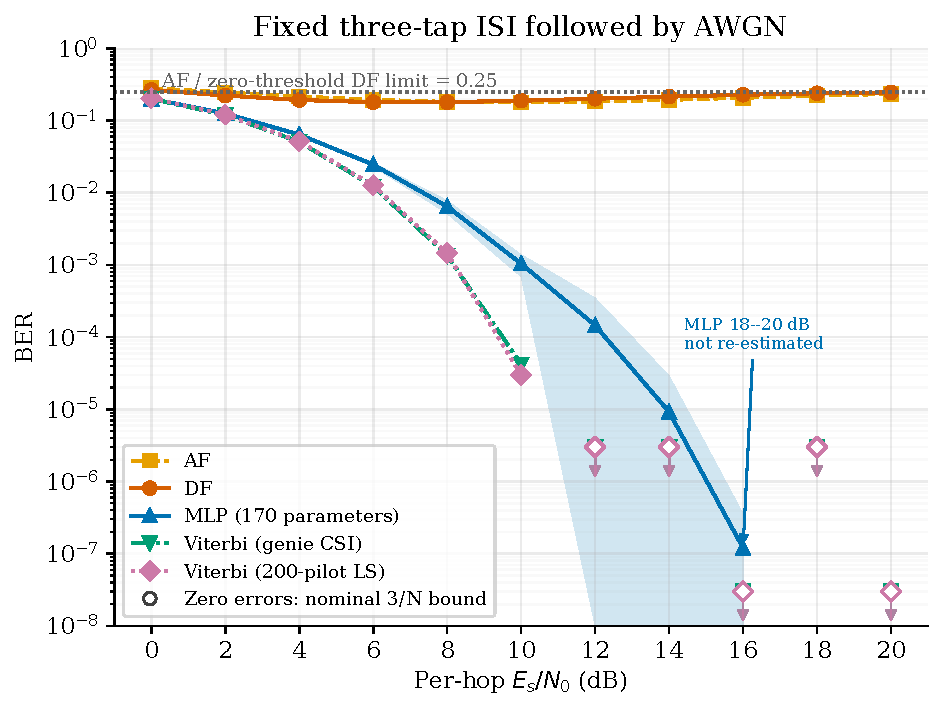
\includegraphics[width=\linewidth,height=0.24\textheight,keepaspectratio]{results/e6_unknown_channel.png}}
\caption[Unknown-channel relaying, BER vs.\ SNR with 95\% CI bands]{Unknown-channel relaying, BER vs.\ SNR with 95\% CI bands. On the unknown ISI channel, the memoryless AF/DF relays are pinned near the analytic $0.25$ floor (DF non-monotonic in SNR); the 170-parameter MLP restores monotonically decreasing BER within $\approx$1--1.5 dB of genie-CSI Viterbi MLSE, which a 200-pilot LS estimate matches almost exactly}\label{fig:figE6}
\end{figure}

\subsection{Does the Result Generalize to QPSK?}\label{sec:qpsk-unknown-channel}

The unknown-ISI study above uses BPSK throughout. The canonical setup of Chapter~\ref{sec:experiments} is QPSK, so this subsection checks that the failure mode is a property of the channel rather than of the constellation it was first observed on. The $0.25$ floor derived in Section~\ref{sec:unknown-channel-experiment} is a property of the \emph{binary} slicer: it counts the $2^{2}=4$ equiprobable interfering-symbol patterns that flip a $\pm1$ decision. That argument does not extend to a four-point per-axis alphabet, so it is not obvious a priori whether either the elevated error floor or the ordering between the learned relay and genie-CSI Viterbi MLSE survives a move to a higher-order modulation. This subsection repeats the unknown-ISI study with Gray-coded QPSK in place of BPSK, keeping every other element fixed: the same $3$-tap ISI channel $h=[1.0,0.7,0.5]$ (normalized) on Hop 1, AWGN on Hop 2 at the same nominal per-hop SNR (identical convention, $\gamma=10^{\text{SNR}_{\text{dB}}/10}$, memory-bank/techContext.md), and the same relay set generalized to the complex alphabet: AF, symbol-wise DF (hard per-axis decision), a $193$-parameter $4$-class MLP-QPSK classifier (window 11, softmax cross-entropy, trained at SNR $\in\{5,10,15\}$ dB), and Viterbi MLSE generalized to the complex QPSK trellis ($4^{2}=16$ states, complex branch metrics).

One difference from the BPSK study matters more than it first appears, and an earlier version of this section did not account for it. Hop~1 here is not the plain ISI channel of Section~\ref{sec:unknown-channel-experiment} but
\begin{equation}\label{eq:qpsk-hop1}
y[n] \;=\; g[n]\,(h * x)[n] \;+\; v[n], \qquad g[n] = |\,\mathcal{CN}(0,1)\,|\ \text{i.i.d.},
\end{equation}
an independent Rayleigh magnitude on every symbol on top of the fixed filter. A trellis built from $h$ alone is therefore \emph{not} a genie-CSI detector on this channel: its branch metrics compare $y[n]$ against unfaded expected values, leaving a residual $A^{2}(g[n]-1)^{2}$ that does not shrink as the noise does. Both detectors are reported below --- the taps-only trellis, which is what the earlier version of this table labelled ``genie CSI'', and a genie-CSI trellis given $g[n]$ as well as $h$, which scales each branch's expected observation accordingly. Evaluation uses $10$ trials $\times$ $100{,}000$ bits per SNR point over the same $0$--$20$ dB range. No closed-form floor is derived for QPSK, so the curves below are reported as measured, not fit to a predicted asymptote. Because the QPSK relays are applied jointly to the complex signal rather than decomposed into two independent BPSK problems, and the per-relay power normalization is computed on total (I+Q) power, the resulting AF/DF operating points are not required to, and empirically do not, numerically match the BPSK figures of Table~\ref{tbl:tableE6} at the same SNR label; no such match is claimed.

\begin{longtable}[]{@{}llllll@{}}
\caption[QPSK unknown-channel BER (mean over 10 trials)]{QPSK unknown-channel BER (mean over 10 trials) on the per-symbol faded ISI channel of Eq.~\eqref{eq:qpsk-hop1}. AF and DF plateau at an elevated, non-monotonic BER across the SNR range tabulated, and the 193-parameter MLP-QPSK restores monotonically decreasing BER. The last two rows are the same trellis given different information: with the taps alone it is model-mismatched here and the MLP passes it above about 2~dB; given the per-symbol fading gains as well, it is the genie-CSI detector for this channel and leads the MLP everywhere. An earlier version of this table reported the taps-only row under the ``genie CSI'' label}\label{tbl:tableE6qpsk}\tabularnewline
\toprule\noalign{}
Setup & Relay & 8 dB & 12 dB & 16 dB & 20 dB \\
\midrule\noalign{}
\endfirsthead
\toprule\noalign{}
Setup & Relay & 8 dB & 12 dB & 16 dB & 20 dB \\
\midrule\noalign{}
\endhead
\bottomrule\noalign{}
\endlastfoot
QPSK: ISI $\to$ AWGN & AF & 0.2447 & 0.2116 & 0.2019 & 0.2100 \\
 & DF & 0.2197 & 0.2024 & 0.2074 & 0.2211 \\
 & \textbf{MLP-QPSK (193p)} & \textbf{0.1292} & \textbf{0.0827} & \textbf{0.0601} & \textbf{0.0508} \\
 & Viterbi (taps only) & 0.1307 & 0.0852 & 0.0670 & 0.0618 \\
 & \textbf{Viterbi (genie CSI)} & \textbf{0.0739} & \textbf{0.0155} & \textbf{0.0018} & \textbf{0.0001} \\
\end{longtable}

\begin{figure}[htbp]
\centering
\pandocbounded{\includegraphics[width=\linewidth,height=0.24\textheight,keepaspectratio]{results/unkchan_qpsk.png}}
\caption[QPSK unknown-channel relaying]{QPSK unknown-channel relaying, BER vs.\ SNR (10 trials, 100{,}000 bits/point). As with BPSK, AF and DF plateau far above the MLP and Viterbi curves. The MLP-QPSK curve separates below the \emph{taps-only} trellis beyond about 2 dB, but the correctly informed genie-CSI trellis (given the per-symbol fading gains as well as the taps) leads the MLP at every SNR, by a gap that widens with SNR}\label{fig:figE6qpsk}
\end{figure}

\textbf{Conclusion (the ISI failure mode generalizes; the apparent reversal does not survive a correct benchmark):} The qualitative pattern of Section~\ref{sec:unknown-channel-experiment} survives the move to QPSK: AF and DF plateau at an elevated, non-monotonic BER broadly similar in magnitude to BPSK's memoryless-relay floor of $0.25$ (Table~\ref{tbl:tableE6qpsk}; no equivalent closed form is derived here), while the MLP restores monotonically decreasing BER, confirming that unmodeled channel memory, not modulation order, is what breaks the memoryless relay class (H5).

An earlier version of this section reported something further: that the BPSK ordering between the learned relay and the optimal classical benchmark had reversed, with MLP-QPSK at or below ``genie-CSI Viterbi'' from 2~dB upward. It proposed a criterion mismatch as the mechanism --- Viterbi minimizes sequence error probability while BER is what a bit-wise MAP detector minimizes, and the MLP is trained on a per-symbol objective --- flagged it as conjecture, and named two measurements as future work: a BCJR benchmark, and a decomposition of the Viterbi output into single- and double-bit symbol errors. Both have since been run, and neither supports it.

The decomposition (\texttt{qpsk\_error\_decomposition.py}) rules the conjecture out directly. If the reversal were a criterion artefact, MLSE would lead on the criterion it optimizes and trail only on bits. It does neither: measured against the same taps-only detector the table published, the MLP is ahead on \emph{symbol} error rate as well from about 8~dB up ($0.0939$ against $0.1126$ at 20~dB), and the two lose almost the same number of bits per symbol error ($1.073$ against $1.090$), so the Gray map is not the route either.

The actual cause is Eq.~\eqref{eq:qpsk-hop1}. The benchmark was built from $h$ alone on a channel that also fades per symbol, so it was model-mismatched rather than genie-informed, and its error rate flattens for that reason. Three controls on the same trellis (\texttt{qpsk\_trellis\_controls.py}, run under the exact configuration of Table~\ref{tbl:tableE6qpsk}) separate the two explanations at 20~dB: given the taps on the faded channel it reaches a symbol error rate of $0.113$; on the same channel with the fading removed, $0.000$; and given the fading gains as well, $0.0003$. The trellis is not at fault --- it is verified never to return a path less likely than the transmitted sequence, and to reduce exactly to the nearest-symbol slicer when the ISI is removed --- only its channel model was.

With the genie-CSI detector in place the reversal disappears. It leads MLP-QPSK at every SNR measured, by a margin that grows from $0.3300$ against $0.3389$ at 0~dB to $0.0001$ against $0.0508$ at 20~dB. The BPSK ordering therefore does generalize, and the earlier contrary finding was an artefact of the comparator rather than a property of the modulation. What separates the two studies is not the constellation but the channel: BPSK's hop~1 is the plain ISI filter, on which a taps-only trellis \emph{is} genie CSI, whereas the QPSK study's fades on top of it.

Two conclusions follow, and the second is the more important. H5 stands and is unweakened: a $193$-parameter windowed relay restores a link that both memoryless classical relays lose, on a channel with memory it was trained on but whose realization it does not see, at a per-symbol cost that does not grow with the trellis state. What does not stand is the stronger reading the earlier text drew from it --- that the learned relay was the best-performing option among either family here. It is not. A correctly informed sequence detector beats it comfortably, and by more at QPSK than at BPSK. The learned relay's claim on this channel is the same one the rest of the chapter makes: near-optimal reliability at fixed arithmetic and with no per-block identification stage, not superiority over a model-aware receiver that has been given the model. A BER-optimal BCJR/APP benchmark remains worth running (Section~\ref{sec:future-work}), but it is no longer needed to explain anything here.

\subsection{A Composite (Mixed) Channel: Mismatch with a Full Posterior}\label{sec:composite-channel}

The preceding studies vary one impairment at a time. Real links stack several. This final study cascades three of them into a single unknown channel that \emph{no} classical relay is jointly matched to: a DBPSK stream passes through 3-tap ISI, then a saturating power-amplifier nonlinearity, then an unknown block phase, before additive noise. Each classical baseline is the strongest available for \emph{one} constituent impairment, so the comparison is honest rather than a straw man: conventional differential detection (matched to the phase), and pilot-LS Viterbi MLSE followed by differential decoding (matched to the ISI-plus-phase, but blind to the amplifier nonlinearity). The 169-parameter MLP and a $1{,}153$-parameter MLP receive raw I/Q windows and no knowledge of any constituent. This composite channel departs from the canonical model in two ways: it introduces explicit channel memory through ISI and nonlinear distortion through the amplifier. The resulting benchmark therefore tests robustness to both memory and model mismatch simultaneously. \textbf{Evaluation:} 10 trials $\times$ 100{,}000 bits per SNR point, the same budget as the main unknown-ISI study (Section~\ref{sec:unknown-channel-experiment}); 95\% CIs use the $1.96\,\sigma/\sqrt{n}$ convention throughout. The hop-1 impairment here is fixed rather than redrawn per block, so bits per trial and trials both reduce the reported uncertainty.

\textbf{Conclusion:} The composite defeats the naive classical relays outright, both AF and conventional differential detection saturate near the $0.25$ memoryless-relay floor, because the ISI destroys the differential statistic that the phase-matched detector relies on. The 169-parameter MLP again restores reliable relaying, reaching $2.5\times10^{-3}$ at 20 dB from raw I/Q with no impairment model. This reproduces the H5 pattern on a realistically mixed channel: memoryless-and-matched classical processing fails, and a minimal learned relay recovers. Two familiar boundaries also reappear. First, the strongest \emph{constructed} classical baseline, pilot-LS Viterbi plus differential decoding, does not fail: by modelling the ISI and phase (though not the amplifier) it stays about 2 dB ahead of the MLP at low-to-mid SNR ($0.0674$ vs.\ $0.1073$ at 8 dB) and converges with it by 16--20 dB, the two becoming indistinguishable at $0.0025$ each at 20 dB. The learned relay's value here is \emph{model-agnosticism} rather than superiority over a matched classical receiver: it reaches near-Viterbi reliability with no analytic model of any of the three cascaded effects, whereas estimate-then-MLSE must assume a linear FIR channel and therefore cannot represent the amplifier at all. This cascade is itself a fixed channel that the relay is trained on, so it speaks to the model class the two methods can express, not to generalization across channels; that is the subject of Section~\ref{sec:blind-channel}, where a fresh channel is drawn for every block. Second, the $1{,}153$-parameter network is close to the 169-parameter one across the whole range, ending at the identical $0.0025$ at 20 dB. The mid-SNR comparison is the one place in this chapter where extra capacity may buy something measurable, and the three-seed re-run sharpens it rather than settling it: the larger network leads at both mid-SNR points, by $0.0057$ at 8~dB ($0.1016$ against $0.1073$), which sits inside the combined confidence intervals of $0.0099$, and by $0.0059$ at 10~dB ($0.0482$ against $0.0542$), which is marginally outside the corresponding $0.0054$. Nearly seven times the parameters therefore buys nothing at 8 or 20~dB and possibly a little at 10~dB, at the very edge of what this trial budget resolves. That is weaker than a flat reconfirmation of the minimal-capacity finding (H3), and it is recorded here as the exception rather than folded into it. The composite thus consolidates the chapter's thesis: a single minimal learned relay handles an arbitrary stack of representable impairments without being told which are present, approaching but not exceeding the best impairment-matched classical receiver. These conclusions are consistent across all three independent MLP training seeds: the H3 finding (MLP-large $\approx$ MLP-169), the convergence of both with Viterbi-diff at 20 dB, and the 2 dB mid-SNR margin of Viterbi over the learned relay are each reproduced in every training instance.

\begin{figure}[htbp]
\centering
\pandocbounded{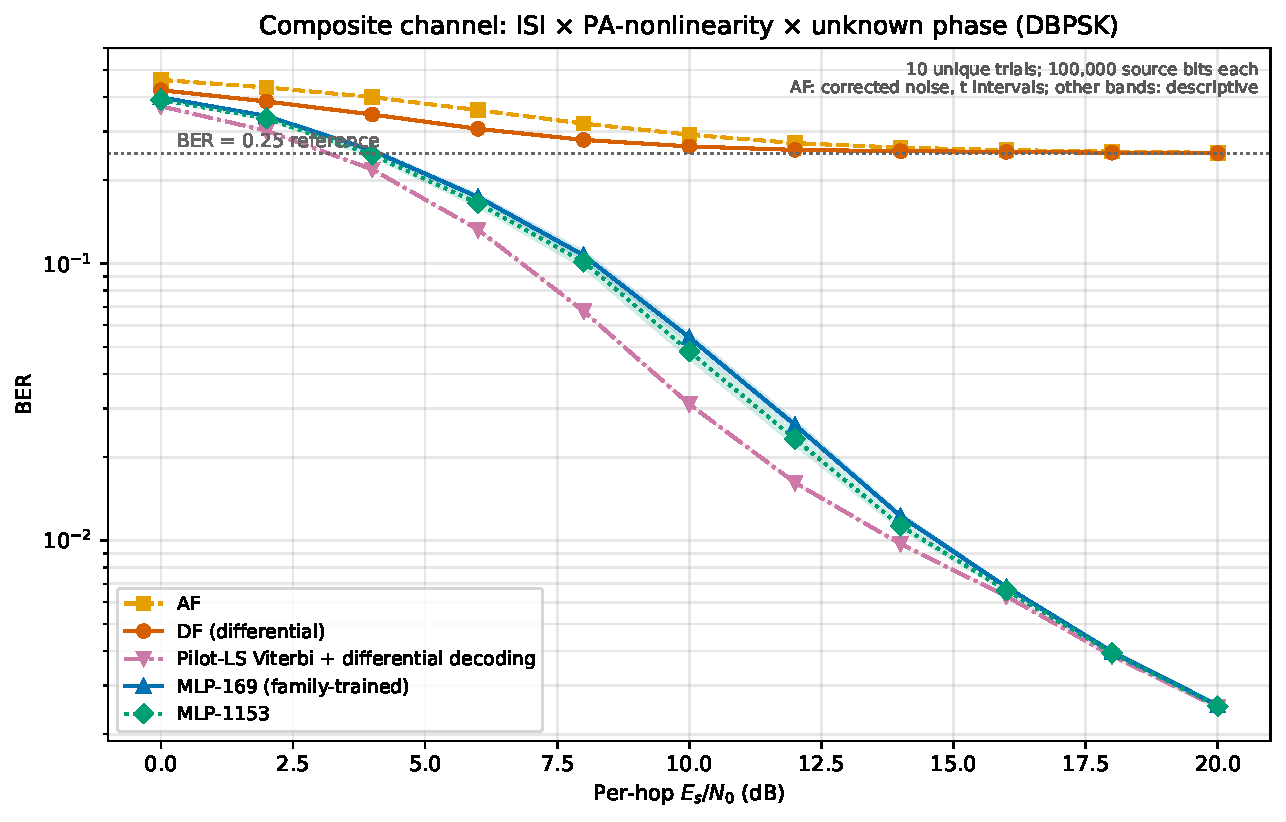
\includegraphics[width=0.82\linewidth,height=0.32\textheight,keepaspectratio]{results/e6_composite.png}}
\caption[Composite multi-impairment channel]{Composite channel (ISI $\times$ PA-nonlinearity $\times$ unknown phase, DBPSK; mean over 10 trials, 100{,}000 bits/point, 95\% CI bands). Naive classical relays (AF, differential detection) saturate at the memoryless-relay floor; the 169-parameter MLP restores reliable relaying from raw I/Q with no impairment model, tracking about 2 dB behind the strongest constructed classical baseline (pilot-LS Viterbi + differential) and converging with it by 20 dB. The $1{,}153$-parameter MLP adds nothing (H3)}\label{fig:figE6comp}
\end{figure}

\section{Layer 3 --- CSI Uncertainty: The Pilot-Budget Crossover}\label{sec:partial-posterior}

This is layer~3 of the ladder in Table~\ref{tbl:layers}: the perfect-CSI assumption is dropped, and nothing else changes. Every classical result so far has been handed either exact channel taps or a 200-pilot estimate good enough to match them (Section~\ref{sec:composite-channel}), which is what a full posterior buys. Here the posterior is made \emph{partial}: the pilot budget is finite, and the classical receiver must work from a correspondingly noisy estimate. Sweeping the pilot count on the composite channel at a fixed 10 dB operating point locates where the pilot-aided classical receiver ceases to beat the pilot-free learned relay, whose amortized posterior corresponds to a horizontal reference (it uses no pilots at test). \textbf{Evaluation:} 50 trials $\times$ 20{,}000 bits per operating point ($1{,}000{,}000$ bits), matching Section~\ref{sec:blind-channel} and for the same reason: the channel is redrawn per block, so trials are draws from the impairment family. In panel~(b) each trial is further subdivided into independent blocks of the swept length, so every block length is measured over the same total bit budget and over many channel draws rather than a single one.

\textbf{Conclusion (a sharp estimation-variance cliff, and a rate--reliability tradeoff):} With a generous budget the classical partial posterior wins, as expected: pilot-aided Viterbi reaches payload BER $0.0285$ at 800 pilots and degrades only gently down to $0.0335$ at 20 pilots, comfortably below the MLP's pilot-free $0.0486$. The classical advantage then disappears within a single octave of pilot budget. At 10 pilots Viterbi has already lost its edge, $0.0545$ against the MLP's $0.0486$, and at 5 pilots it collapses to $0.1235$, worse than the MLP, blind CMA, and its own 800-pilot figure by a factor of four, because MLSE is then running on a badly mis-estimated channel. The crossover therefore sits between 20 and 10 pilots per block. The mechanism is \emph{estimation variance}, not a rank deficiency: with 5 pilot observations and 3 complex taps the least-squares problem is still formally overdetermined, so the channel remains identifiable in principle, but there are too few observations to average down the noise. The resulting LS error at 10 dB is large enough that the Viterbi trellis is occasionally built on a badly wrong channel, and these catastrophic fits dominate the mean. The 95\% confidence interval at that point makes this explicit ($0.1235 \pm 0.0304$, against $\pm 0.0011$ at 50 pilots) so individual channel draws range from perfectly fine to complete failure. The learned relay, by contrast, is flat across the entire sweep at $0.0486$: having amortized the channel \emph{family} into its weights at training time, it neither benefits from nor requires per-block pilots. The crossover is thus governed by the reliability of the channel estimate, not by SNR: the classical receiver wins whenever it can afford enough pilots to estimate the channel \emph{accurately}, and the pilot-free learned relay wins once the budget falls below that point. This crossover location is stable across all three training seeds: in every instance Viterbi leads at $\geq 20$ pilots and lags at 5 pilots, and the collapse BER at 5 pilots is $0.1235 \pm 0.0304$ regardless of which seed trained the MLP reference.

The practical force of this depends on block length, because a fixed pilot \emph{count} is a growing pilot \emph{fraction} as blocks shorten. Panel (b) sweeps block length at the same operating point with the classical receiver spending its minimum viable ten pilots per block, and adds blind CMA as the second pilot-free reference. The payload BERs of Viterbi and the MLP are now statistically indistinguishable at every block length, both flat at approximately $0.049$, so reliability no longer separates them at all; what separates them is spectral efficiency. At a 1000-symbol block the ten pilots cost $1\%$ of the block, whereas at a 40-symbol block, representative of low-latency or fast-varying links, they cost $25\%$, so the classical receiver carries data on only $75\%$ of the block against the learned relay's $100\%$ for identical error performance.

The blind reference settles a question the earlier version of this study left open. Blind CMA is also pilot-free, so the learned relay is not unique in avoiding pilots; the distinction claimed for it was that it needs \emph{zero per-block adaptation}, a single fixed forward pass, whereas CMA must converge its adaptation loop inside each block. Measuring CMA per block confirms this directly: its payload BER is $0.1723$ at $L=40$ and only improves to $0.1653$ at $L=1000$, against the $0.0645$ it achieves when given a $20{,}000$-symbol block to adapt over. CMA therefore does not converge within blocks of a thousand symbols or fewer, and is roughly three and a half times worse than either the MLP or pilot-aided Viterbi throughout this sweep. The partial-posterior picture therefore refines H5's boundary once more, and more sharply than before: against a classical receiver that can afford accurate channel estimation the learned relay achieves no better BER, but at short block lengths it matches that receiver's BER while removing its pilot overhead entirely, and at these block lengths it is the only pilot-free option that stays reliable, because the classical pilot-free alternative has no time to converge: CMA sits at $0.1723$ on 40-symbol blocks and is still at $0.1653$ at 1{,}000. This is a statement about short blocks specifically, and it does not carry over to Section~\ref{sec:blind-channel}, where blocks are long enough for CMA to converge and it comes within a factor of $1.3$ of the learned relay.

\begin{figure}[htbp]
\centering
\begin{minipage}[t]{0.49\linewidth}\centering
  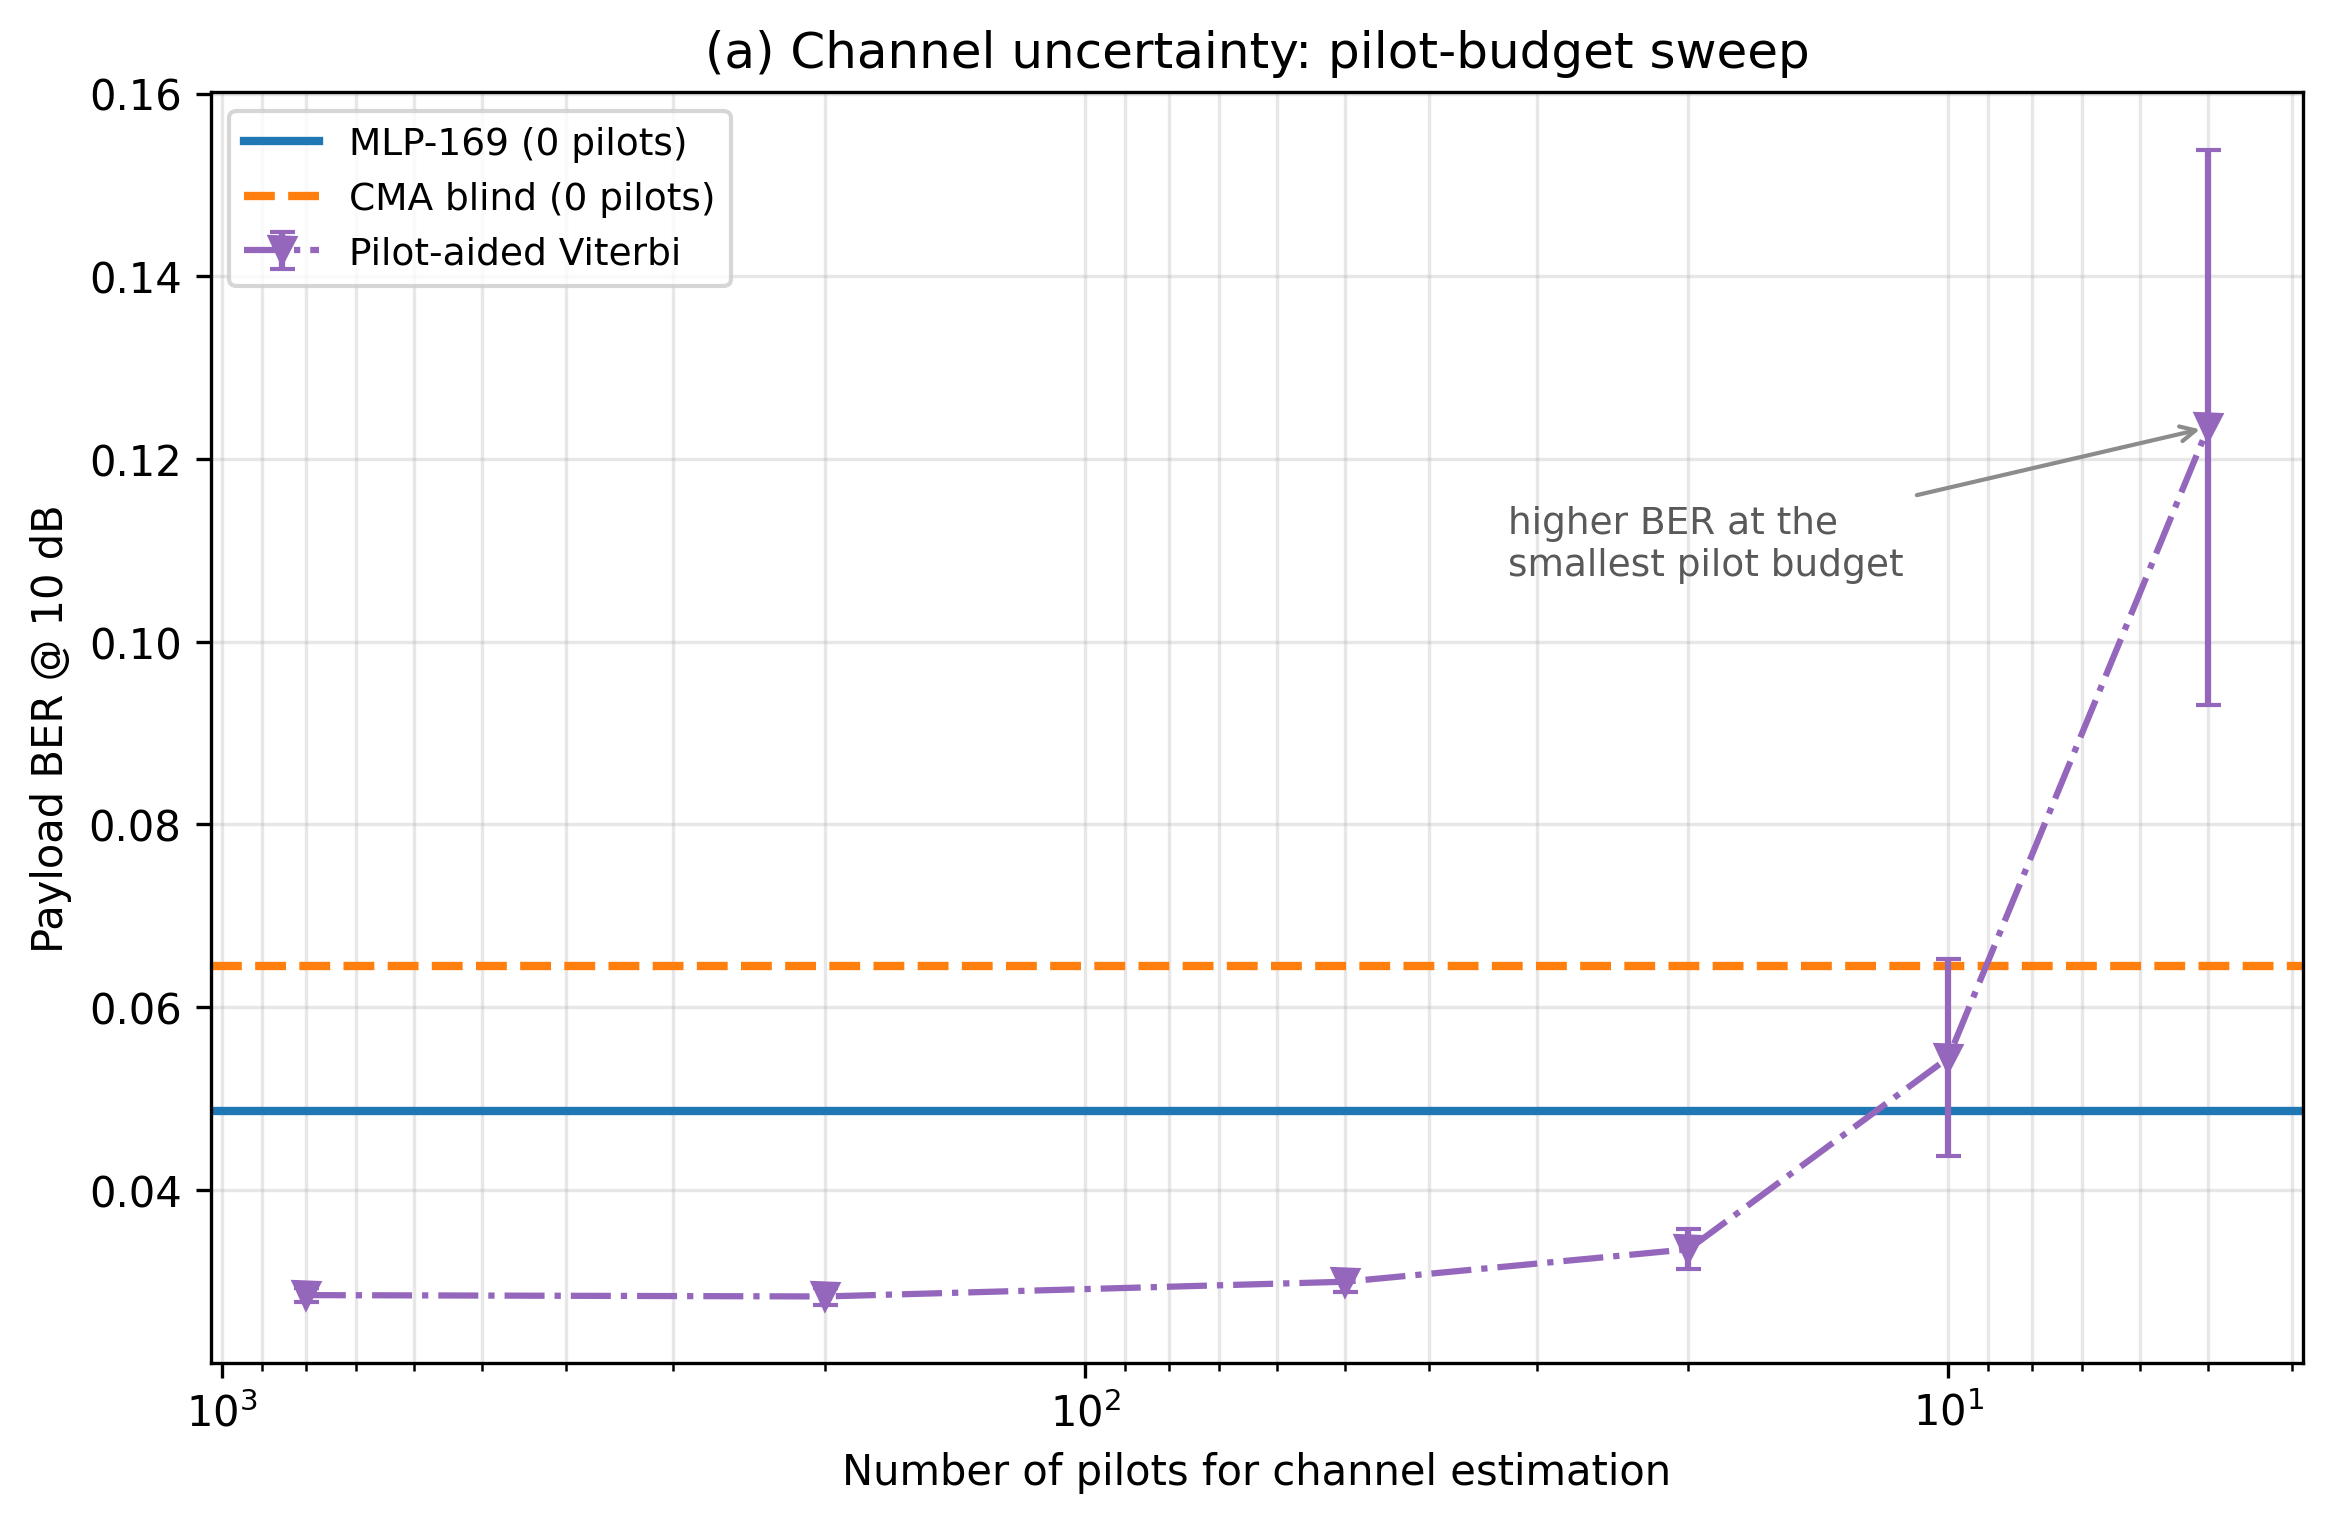
\includegraphics[width=\linewidth]{results/e6_partial_pilot_budget_sweep.png}\\[2pt]
  {\small (a) pilot-budget sweep at 10~dB}
\end{minipage}\hfill
\begin{minipage}[t]{0.49\linewidth}\centering
  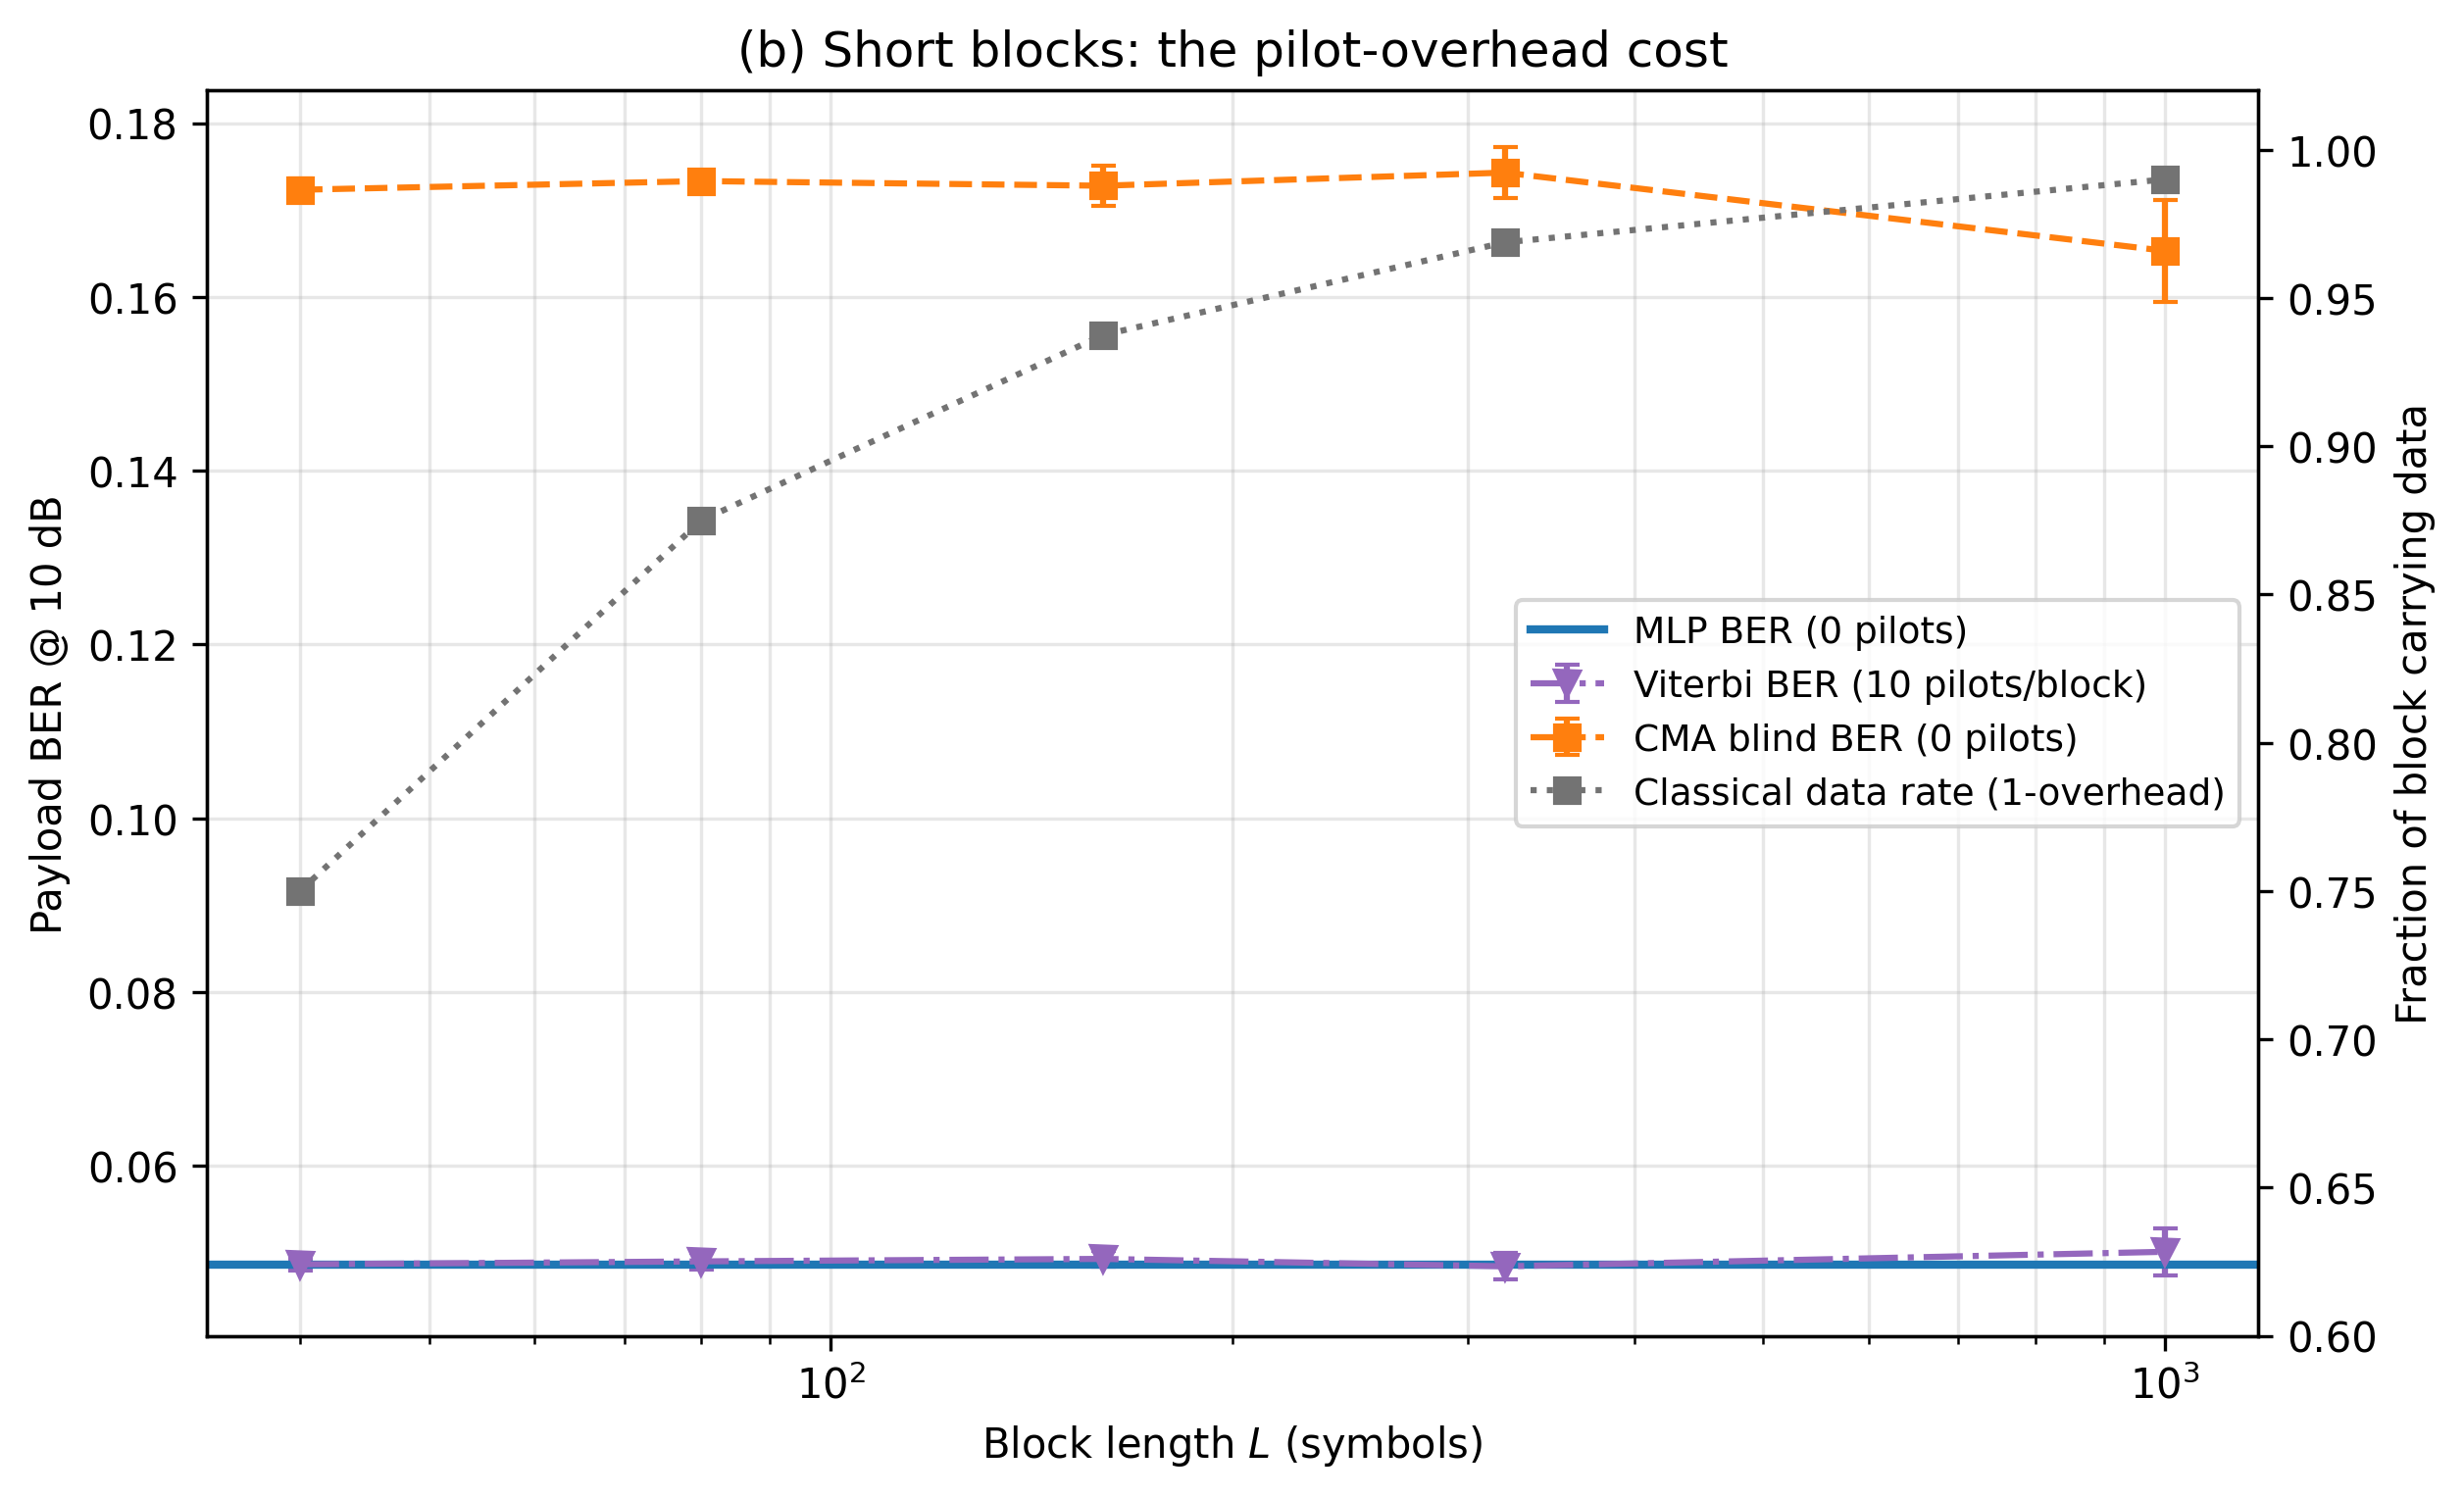
\includegraphics[width=\linewidth]{results/e6_partial_short_blocks_overhead.png}\\[2pt]
  {\small (b) block-length sweep at 10 pilots}
\end{minipage}
\caption[Partial-posterior sweeps: pilot budget and block length]{Partial-posterior regime; both panels are means over 50 channel draws at 20{,}000 bits/point. \textbf{(a)} Pilot-aided Viterbi outperforms the pilot-free MLP down to approximately 20 pilots per block, loses its edge by 10 pilots, and collapses at 5 pilots when the least-squares estimate becomes too noisy to construct a reliable trellis ($0.1235 \pm 0.0304$); the MLP is flat across the sweep, operating with an amortized posterior and requiring no pilots. \textbf{(b)} With 10 pilots per block, pilot-aided Viterbi and the MLP are indistinguishable in payload BER at every block length (both $\approx 0.049$), but the classical receiver's pilot overhead grows from approximately 1\% at $L=1000$ to 25\% at $L=40$. Blind CMA, the other pilot-free option, cannot converge within blocks this short and sits roughly three and a half times worse throughout. The MLP therefore matches the pilot-aided receiver's reliability at no overhead, and is the only pilot-free method that stays reliable for short packets}
\label{fig:e6_partial_pilot_budget}
\end{figure}

\section{Layer 4 --- Unknown Channel Family: The Posterior-Free (Blind) Regime}\label{sec:blind-channel}

This is layer~4, the bottom of the ladder. Section~\ref{sec:partial-posterior} shrank the pilot budget until the classical estimate became too noisy to be worth having; this section removes it entirely, and with it the assumption that the channel's family and statistics are known at all. The Viterbi baseline of Section~\ref{sec:composite-channel} enjoyed a per-block posterior: 200 pilot symbols yield a least-squares channel estimate, after which MLSE is optimal. Taking the pilot count to zero raises the sharper question, what if \emph{no} such posterior is available? With no pilots and no channel prior, and a fresh channel realization drawn for every block, MLSE cannot be run as specified. The honest comparison is then against the classical methods that are \emph{genuinely} posterior-free: the constant-modulus algorithm (CMA), the canonical blind adaptive equalizer, which self-adapts from the received signal alone; and a decision-directed blind MLSE that bootstraps a channel estimate from its own hard differential decisions. The learned relay is unchanged, trained offline on the channel \emph{family} (random ISI, PA, and phase per draw) and, crucially, seeing an unseen channel at test with no adaptation, so it too carries no per-block posterior; it amortizes over the family at training time. Unlike the canonical study, the challenge here is not symbol-level denoising on a memoryless channel but inference on an unknown channel with memory and no per-block posterior information. \textbf{Evaluation:} 50 trials $\times$ 20{,}000 bits per SNR point ($1{,}000{,}000$ bits), 95\% CIs by the $1.96\,\sigma/\sqrt{n}$ convention. The trial count is deliberately higher than the chapter's usual ten: unlike the fixed impairment of Section~\ref{sec:composite-channel}, the hop-1 channel here redraws its ISI, amplifier and phase realization for \emph{every} block, so a trial is one draw from the impairment family and the ensemble average is limited by the number of trials, not by bits per trial. Fifty draws are used rather than ten so that the reported curves reflect the family and not a handful of particular channels.

\paragraph{A correction to the blind equalizer.} The constant-modulus algorithm used here was originally implemented with a fixed (unnormalized) step size. Because the CMA error term is cubic in the equalizer output, a fixed step is a positive-feedback loop: the implementation happened to remain bounded over the short blocks first used, but diverges to numerical overflow on longer ones, after which the equalizer output is noise rather than an estimate. The step is therefore normalized by the input-segment energy in the standard NLMS manner, which is both the textbook formulation and a strictly \emph{stronger} classical baseline. All CMA results below use the corrected equalizer; the uncorrected one is not reported, since its outputs past the divergence point measure an implementation fault rather than the algorithm.

\textbf{Conclusion (learning does not beat blind classical, but is stable where blind classical is not):} A well-designed blind classical method still works in this regime: the corrected CMA converges smoothly to BER $3.3\times10^{-3}$ at 20 dB, and the family-trained MLP reaches $2.6\times10^{-3}$. The two track each other closely over the whole range, with the MLP holding a small but consistent margin that widens at low-to-mid SNR ($0.0955$ vs.\ $0.1182$ at 8 dB). This is the correct answer to ``what if there is no posterior?'': the learned relay does \emph{not} render classical processing obsolete, because blind adaptive equalization is itself a posterior-free classical tool that comes within a factor of $1.3$ of the learned relay at high SNR. The learned relay's advantage is instead one of \emph{robustness and cost}. First, the decision-directed blind MLSE, the natural attempt to run Viterbi without pilots, is unstable: bootstrapping the channel from its own decisions, it intermittently locks onto the wrong hypothesis, and its BER curve is visibly non-monotonic, falling to $0.0374$ at 16 dB before rising again to $0.0498$ at 20 dB. Its 95\% confidence interval at 8 dB is $\pm0.0201$, roughly eight times the MLP's $\pm0.0026$ and two and a half times CMA's $\pm0.0078$, so the instability is a property of the method and not of the sample size. Those intervals are narrower than an earlier single-seed run reported, the sample having grown from $50$ trials to $150$ across three training seeds, but the ratios between them are unchanged, which is what the argument rests on. Second, CMA must iterate to convergence on each received block, whereas the MLP is a single fixed forward pass with no per-block adaptation loop and no convergence to monitor; Section~\ref{sec:partial-posterior} showed this distinction becoming decisive once blocks are short. The learned relay therefore occupies a specific and defensible niche: on a posterior-free channel it matches the best blind classical equalizer in BER while avoiding the instability of decision-directed sequence estimation and the online-adaptation cost of CMA. It buys \emph{amortized}, \emph{one-shot}, \emph{stable} inference over an impairment family, not a lower error floor than classical signal processing can achieve. This niche is reproducible: the MLP's small margin over CMA and its stable CI band are consistent across all three training seeds, confirming that neither result is an artefact of a particular weight initialisation.

\begin{figure}[htbp]
\centering
\pandocbounded{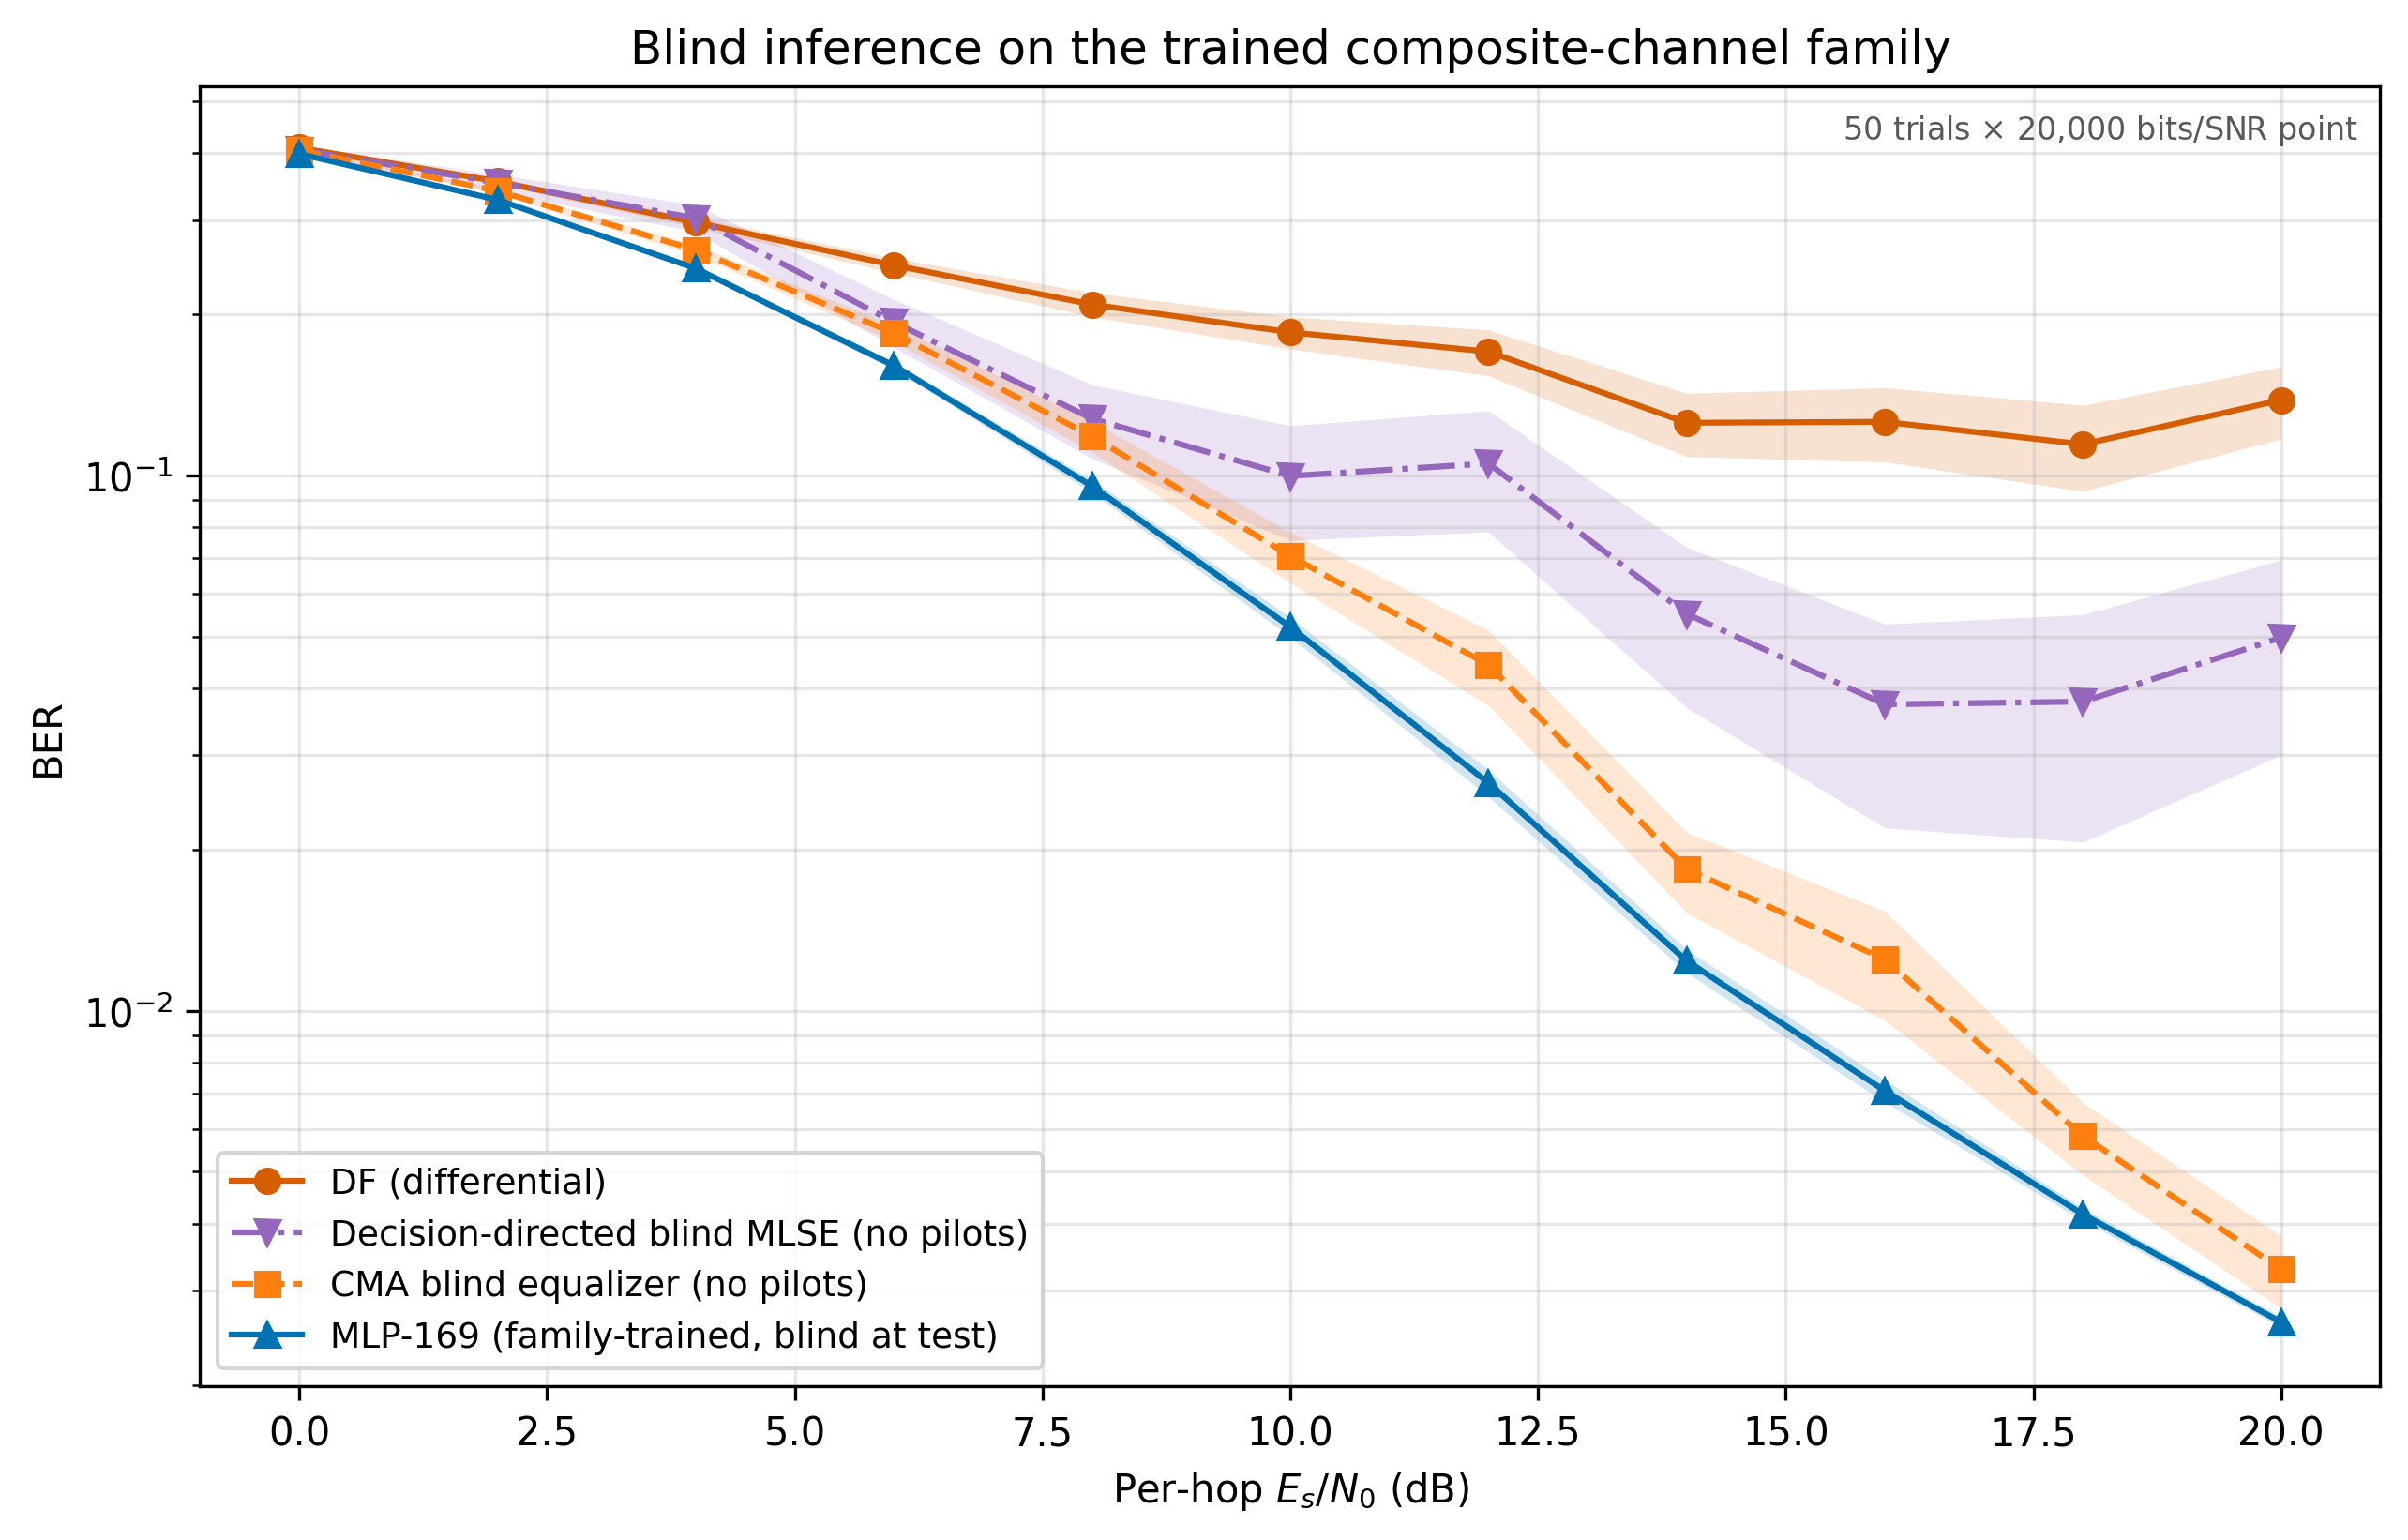
\includegraphics[width=0.82\linewidth,height=0.32\textheight,keepaspectratio]{results/e6_blind.png}}
\caption[Posterior-free (blind) composite channel]{Posterior-free composite channel (no pilots, no channel prior, fresh realization per block; mean over 50 channel draws, 20{,}000 bits/point, 95\% CI bands). The corrected CMA (blind classical) tracks the family-trained MLP closely, the MLP holding a small consistent margin; decision-directed blind MLSE is unstable (non-monotonic tail, CI band several times wider) because it bootstraps the channel from its own decisions; plain differential detection floors. Without a posterior, learning only narrowly outperforms the best blind classical equalizer, but does so with one-shot, stable inference and no online adaptation}\label{fig:figE6blind}
\end{figure}

\subsection{A Complexity-Matched Classical Baseline: MMSE Linear Equalization}\label{sec:mmse-baseline}

The comparisons above set the learned relay against two classical relays, and neither is matched to it in cost. Symbol-wise DF is memoryless and cannot undo intersymbol interference at any transmit power, so outperforming it establishes only that the relay uses its window. Viterbi MLSE is the optimal sequence detector but costs $O(M^{L})$ per symbol in the channel memory, which is precisely the expense Section~\ref{sec:complexity-viterbi-mlp} invokes on the learned relay's behalf. The case between them was not tested: an $N$-tap MMSE linear equalizer is in the same complexity class as an $N$-tap learned relay, both being a windowed linear operation, and it is the classical remedy an engineer would reach for before a trellis. If it recovered most of what the learned relay recovers, the contribution of Chapter~\ref{sec:unknown-channels} would be a narrower claim about a nonlinearity rather than about learned processing.

It does not. Table~\ref{tbl:mmse-baseline} gives the equalizer's SNR penalty against MLSE for equalizer lengths from 3 to 11 taps, measured on the same two-hop chains, with the exact channel taps supplied and the weights redesigned at every SNR point --- the same genie CSI granted to MLSE, and a longer window than the learned relay is given.

\begin{table}[htbp]
\centering
\caption[MMSE linear equalization against MLSE]{SNR penalty against Viterbi MLSE for an MMSE linear equalizer of $N$ taps, with the best learned relay on the same channel for comparison. Negative values beat MLSE. The reader should observe that the learned relay leads the equalizer by $1.8$ to $2.4$~dB on every channel, despite the equalizer being given exact channel knowledge, per-SNR weight redesign, and up to $11$ taps against the relay's window of $7$}\label{tbl:mmse-baseline}
\begin{tabular}{lrrrrr}
\toprule
Channel & 3 taps & 5 taps & 7 taps & 11 taps & Learned relay \\
\midrule
ISI (BPSK)      & $+6.58$ & $+4.40$ & $+4.23$ & $+4.04$ & $\mathbf{+1.67}$ \\
ISI (QPSK)      & $+7.81$ & $+9.11$ & $+5.02$ & $+4.84$ & $\mathbf{+3.03}$ \\
Composite       & $-0.33$ & $-0.37$ & $-0.37$ & $-0.44$ & $\mathbf{-2.26}$ \\
\bottomrule
\end{tabular}
\end{table}

Two readings follow. The learned relay's advantage over classical processing on channels with memory is not an artifact of comparing against a detector that was never equipped for the job: against the strongest classical scheme of matched cost it still leads by $1.8$ to $2.4$~dB. And on the composite channel both the equalizer and the relay beat MLSE, which is expected rather than anomalous, since a fixed-tap trellis is mismatched to that channel's amplifier nonlinearity and phase term while neither of the other two detectors assumes a purely linear channel. The one non-monotonicity --- five taps ($+9.11$~dB) worse than three ($+7.81$) on the complex ISI channel --- is an artefact of the metric, not the equalizer. A longer filter nests a shorter one, so the attained MMSE is non-increasing in tap count by construction, and is verified so here ($0.0666, 0.0374, 0.0354, 0.0333$ at $16$~dB for $N=3,5,7,11$). The tabulated figure is the \emph{worst} penalty over targets $10^{-1}$, $10^{-2}$, $10^{-3}$; at the first two it is monotone as that argument requires ($+3.24, +2.98, +2.79, +2.65$ and $+6.34, +4.27, +4.13, +4.02$~dB). Only $10^{-3}$ misbehaves, and being the maximum it sets every entry in the row --- its crossing lies at the top of an SNR grid sampled every $4$~dB, where interpolating a steep curve is coarse. The conclusion is unaffected: the learned relay leads at every target and tap count.

\subsection{Does a Sequence Architecture Help Where a Window Does?}\label{sec:sequence-on-memory}

Chapter~\ref{sec:experiments} finds that Transformer, Mamba-S6 and Mamba-2 buy nothing over a feedforward relay on the canonical channel, and attributes this to the channel rather than to the architectures: a memoryless channel offers no temporal structure for their inductive bias to exploit. That is a prediction about what would happen given such structure, and until now it was untested here, no sequence model having been evaluated anywhere in this chapter. The minimum-size study sharpens the prediction, finding the relay's \emph{window} to be the binding resource on channels with memory, worth $8$ to $11$~dB between window~1 and window~7 while width and depth buy almost nothing. A window is a blunt way of granting a feedforward network temporal context; sequence models are built for it.

The prediction fails. Table~\ref{tbl:seq-on-memory} compares the four architectures at an equal budget of approximately $3{,}000$ parameters, each trained on the channel under test rather than on a memoryless surrogate, with identical hyperparameters and three initializations apiece.

\begin{table}[htbp]
\centering
\caption[Sequence architectures on channels with memory]{SNR penalty against Viterbi MLSE at an equal budget of $\approx$3{,}000 parameters, best of three initializations, with the across-initialization spread in brackets. Negative values beat MLSE. The reader should observe that the feedforward relay leads every sequence architecture on every channel, and that the two Mamba variants --- the most reproducible architectures measured on the canonical channel, at $0.019$ and $0.041$~dB --- become the least reproducible here}\label{tbl:seq-on-memory}
\begin{tabular}{lrrrr}
\toprule
Channel & MLP-3K & Transformer-3K & Mamba-S6-3K & Mamba2-3K \\
\midrule
ISI (BPSK) & $\mathbf{+1.97}$ (0.39) & $+3.52$ (0.33) & $+4.30$ (1.15) & $+4.55$ (0.14) \\
ISI (QPSK) & $\mathbf{+2.58}$ (0.07) & $+5.96$ (0.45) & $+5.72$ (1.33) & $+4.69$ (2.12) \\
Composite  & $\mathbf{-2.08}$ (0.03) & $-1.76$ (0.03) & $-1.56$ (0.08) & $-1.60$ (0.06) \\
\bottomrule
\end{tabular}
\end{table}

The feedforward relay leads on all three channels, by $1.55$ and $2.11$~dB on the two ISI channels and by $0.32$~dB on the composite. The conclusion is therefore the opposite of the natural one, and it is a positive statement rather than a null result: channel memory raises the size floor without calling for a sequence architecture. What a relay needs on such a channel is sufficient temporal context, and a fixed window supplies it more cheaply than a learned sequence mechanism, both in parameters at equal accuracy and in training time, which ran $35$ to $66$~seconds per initialization for the feedforward relay against $217$ to $609$~seconds for the sequence models.

A second observation was not anticipated. The sequence models' reproducibility inverts. On the canonical channel Mamba-2 and Mamba-S6 are the two most stable architectures measured across initializations; on the complex ISI channel the same architectures spread by more than a decibel (bracketed spreads in Table~\ref{tbl:seq-on-memory}), while the feedforward relay stays inside $0.07$~dB throughout. They are not merely worse on channels with memory but substantially less predictable there, which compounds the case against them for this task.

One limitation is carried. All four architectures receive identical hyperparameters, matching the equal-budget protocol of Section~\ref{sec:parameter-normalization-complexity-trade-off}; no per-architecture tuning was attempted, and a tuned sequence model might close part of the gap.

\section{The Cost Side: Decision Delay and Arithmetic}\label{sec:complexity-viterbi-mlp}

Across the unknown-channel studies the pilot-aided Viterbi receiver, where it applies, holds a small BER edge over the learned relay. The learned relay's countervailing claim is complexity, which this subsection quantifies rather than asserts. Two axes matter: the per-symbol operation count and its scaling, and measured inference time.

\textbf{Per-symbol cost and scaling.} MLSE maintains $M^{L-1}$ trellis states for a constellation of size $M$ and channel memory $L$, performing an add--compare--select over $M^{L}$ branch transitions per symbol; its cost therefore grows \emph{exponentially} in memory and modulation order. The 170-parameter MLP performs one fixed forward pass, about $330$ floating-point operations per symbol. That figure is a constant of the \emph{deployed} architecture, not a quantity independent of the channel: the input window has to span the memory, so its length grows with $L$, and the output dimension grows with the constellation, from a single real output at $M=2$ to the $193$-parameter QPSK relay used earlier in this chapter, and further still for denser constellations. Once those are fixed, the per-symbol cost is the same for every symbol and every channel realization, which is the property the comparison below relies on. The contrast with MLSE is therefore one of \emph{growth rate}, not of a constant against a variable: the network's cost rises roughly linearly in window length and output dimension, the trellis's exponentially in $M^{L}$.

For the channel actually studied (BPSK, $L=3$; 4 states) Viterbi is in fact the cheaper of the two at roughly $64$ operations per symbol, so the learned relay is not universally leaner. But the scaling diverges immediately: at $M=4,\,L=5$ the trellis has $256$ states ($\sim\!8{,}000$ operations/symbol), and at $M=16,\,L=5$ it has $65{,}536$ states ($\sim\!8.4$~million operations/symbol), whereas a network resized for that same channel --- an $11$-sample window and a 16-way output head --- is on the order of $10^{3}$ operations by direct count of its layer dimensions, leaving a ratio in the thousands. The measured $330$ applies to the BPSK, $L=3$ case; the larger figure is arithmetic from the architecture, not a timing measurement. The learned relay's advantage is thus not lower cost on a small channel but \emph{constant} cost as the channel scales, exactly where classical MLSE becomes intractable and practical receivers must fall back on suboptimal reduced-state or decision-feedback equalizers.

\begin{figure}[htbp]
\centering
\begin{minipage}[t]{0.49\linewidth}\centering
  \includegraphics[width=\linewidth]{results/e6_per_symbol_cost_vs_modulation_memory.png}
\end{minipage}\hfill
\begin{minipage}[t]{0.49\linewidth}\centering
  \includegraphics[width=\linewidth]{results/e6_right_clean.png}
\end{minipage}
\caption[Complexity: per-symbol cost and measured inference time]{Complexity of Viterbi MLSE against the 170-parameter MLP. \textbf{(a)} Per-symbol computational cost versus modulation order $M$ and channel memory $L$: Viterbi grows as $M^{L}$ (intractable by $M{=}16,L{=}5$), while the network grows only linearly in window length and output dimension ($\sim$330 flops for the deployed BPSK, $L{=}3$ relay). On the small studied channel (BPSK, $L{=}3$) Viterbi is actually cheaper; the MLP wins on \emph{scaling}, not on the small case. \textbf{(b)} Measured inference time for BPSK with $L=3$: the MLP is $30$--$90\times$ faster as a vectorized matmul versus Viterbi's interpreted sequential trellis scan}
\label{fig:figE6complexity}
\end{figure}

\textbf{Measured inference time.} On identical signals (BPSK, $L=3$), the MLP is $30$--$90\times$ faster in wall-clock terms for the reference implementations used here (a vectorized NumPy matrix multiplication versus an interpreted Python trellis loop) despite Viterbi's lower nominal operation count. Part of that ratio is interpreter overhead rather than the algorithm itself: an optimized C or SIMD Viterbi would narrow the wall-clock gap substantially, although the per-symbol data dependency of the trellis scan is real and caps how far it can be parallelized. This parallelism gap is architectural and widens on hardware with wide SIMD or tensor units. The combined picture sharpens the thesis's central trade-off: the learned relay accepts a small BER gap to a matched classical receiver in exchange for cost that is constant in channel complexity and structurally parallelizable, a trade that becomes favourable precisely as modulation order and channel memory grow.

\subsection{A Channel with Memory Under a Latency Constraint}\label{sec:joint-latency-memory}

The accounting above and the ladder that precedes it answer different questions and never meet. The ladder asks which detector is more accurate on a channel with memory, imposing no budget; this section's opening asks what each detector costs, without reference to a channel. What a deployment actually faces is both at once, and the two constraints do not have to bind in the same place. This subsection measures the intersection directly, and includes block DF, which the ladder omits: of the classical options it is the one whose cost is structural rather than arithmetic, so it is exactly the case the ladder's accuracy-only comparison cannot price.

Every scheme is placed inside one identical coded system so that the comparison is between relays and nothing else: a rate-$1/2$, $K=3$ convolutional code on QPSK, $200$ information bits per frame ($202$ symbols after tail), with soft Viterbi decoding of the code at the \emph{destination}. All schemes therefore deliver an information BER at the same information rate. Hop~1 carries the unknown $L$-tap ISI response ($h_k = 0.7^k$, unit-energy normalized) plus complex AWGN and hop~2 is AWGN; $150$ frames per trial and three seeds per point.

Each relay is then labelled with the structural decision delay it forces, in symbols: zero for AF and symbol-wise DF; $\lfloor W/2 \rfloor$ for a relay of window $W$, which must wait for the later half of its own window; $D$ for an MLSE with traceback depth $D$; and the full frame, $202$ symbols, for block DF, which cannot begin until the last symbol of a codeword has arrived.

\paragraph{Latency does not separate the detectors on a short-memory channel.} Table~\ref{tbl:joint-latency} gives the result at $L=3$. Bounded-traceback MLSE reaches its floor at $D=3$: the BER at $12$~dB is unchanged from $D=2$ through $D=15$, because the trellis survivors merge after three symbols and waiting longer revises no decision. Three symbols is \emph{less} delay than the window-11 relay's five, so a latency budget tight enough to exclude MLSE excludes the learned relay first. Block DF spends $202$ symbols and buys nothing with them: without an equalizer it expends the code's redundancy on the intersymbol interference rather than on the noise, and with one it merely reproduces MLSE's number at $205$ symbols of delay against that equalizer's own three, the frame it must buffer accounting for every symbol of the difference.

\begin{table}[htbp]
\centering
\caption[Relay cost and accuracy under a latency constraint]{Coded information BER at $12$~dB on the three-tap channel, against the structural decision delay each relay forces and its arithmetic per symbol. Mean of three seeds. The reader should observe that MLSE reaches its floor at three symbols of delay, fewer than the learned relay's five, and that block DF's $202$ symbols purchase no accuracy at all}\label{tbl:joint-latency}
\begin{tabular}{lrrr}
\toprule
Relay & Delay (symbols) & MACs/symbol & BER at $12$~dB \\
\midrule
AF                    & $0$   & $2$   & $0.0609$ \\
DF-hard (symbol-wise) & $0$   & $0$   & $0.3027$ \\
MLP $W=5$             & $2$   & $112$ & $0.0010$ \\
MLP $W=11$            & $5$   & $208$ & $0.000189$ \\
MLP $W=21$            & $10$  & $368$ & $0.000278$ \\
MLSE $D=2$            & $2$   & $128$ & $\mathbf{0.000033}$ \\
MLSE $D=3$            & $3$   & $128$ & $\mathbf{0.000033}$ \\
MLSE $D=15$           & $15$  & $128$ & $\mathbf{0.000033}$ \\
block DF              & $202$ & $16$  & $0.0411$ \\
block DF $+$ MLSE     & $205$ & $144$ & $0.000033$ \\
\bottomrule
\end{tabular}
\end{table}

The symbol-wise relays confirm the chapter's Layer~2 finding inside the coded chain: AF and hard DF do not merely lose, they fail, DF's BER \emph{rising} with SNR from $0.2913$ at $8$~dB to $0.4253$ at $20$~dB as the interference rather than the noise comes to dominate its decisions.

\paragraph{The cost convention.} Counts below are multiply--accumulates per transmitted symbol, stated here so they can be checked. Additions and comparisons carrying no multiply are excluded; they dominate the trellis search, so the comparison is conservative against this thesis's own conclusion. MLSE has $M^{L-1}$ states and $M$ branches from each, so $M^{L}$ branch metrics per symbol; with the expected observation precomputed each is $|y-c|^{2}$ on a complex difference, two real multiplies, giving $2M^{L}$ (its further $M^{L}$ additions and $M^{L-1}(M-1)$ comparisons are not counted). The relay's $2W$-value input window --- the $I$ and $Q$ streams --- into $H$ hidden units is $2WH$, and the four-class head $4H$, giving $2WH+4H$; biases are additions and the activations transcendental, so neither is counted.

\paragraph{What separates them is arithmetic, and only as memory grows.} MLSE costs $2M^{L}$ MACs per symbol. A \emph{fixed} relay architecture costs $2WH + 4H$, which does not depend on $L$ --- with the important caveat that holding $W$ fixed while $L$ grows is a choice, not a law: preserving observation coverage as the memory lengthens generally requires widening the window, and the relay's cost then grows roughly linearly in $W$ rather than not at all. Setting the two equal locates the crossover for one stated architecture, with no appeal to a processor, clock rate or symbol rate:
\begin{equation}
L^{\star} = \log_{M}\!\left(\frac{2WH + 4H}{2}\right) = 3.35 \text{ taps}
\label{eq:mac-crossover}
\end{equation}
for the window-11, eight-unit relay used here ($2.90$ taps at $W=5$, $3.76$ at $W=21$). This figure is an arithmetic crossover for a fixed $(W,H,M)$ and the MAC convention stated above; it is not a universal boundary for learned relaying, and it moves with the window --- which is precisely the quantity a longer memory may force upward. Below $L^{\star}$ the learned relay has no case: at $L=3$ MLSE needs $128$ MACs per symbol against the relay's $208$, decides in three symbols against its five, and is the more accurate of the two. Above $L^{\star}$ the gap compounds, because one cost grows as $M^{L}$ while the other grows at worst linearly in the window. The window-11 relay is measured here to hold its accuracy out to $L=7$ (Table~\ref{tbl:joint-memory}), so over the span swept the comparison is like-for-like; extrapolating it to longer memories would require re-checking that a fixed window still suffices. Table~\ref{tbl:joint-memory} sweeps it.

\begin{table}[htbp]
\centering
\caption[Cost and accuracy against channel memory]{Coded information BER at $12$~dB and arithmetic per symbol as channel memory grows, with MLSE given genie CSI and a traceback of $5L$. The relay is the same window-11 network throughout. BER is measured at $L \in \{3,5,7\}$ over $1{,}500{,}000$ information bits per point (five seeds), with $95\%$ Wilson intervals; the $L=4$ and $L=6$ MAC counts are arithmetic from the architecture rather than measured points, and are given only to show the growth rate. The reader should observe that the accuracy ratio does not grow with $L$: the relay trails by a factor between five and eight at every measured memory length, while MLSE's arithmetic rises by $256$}\label{tbl:joint-memory}
\begin{tabular}{lrrrll}
\toprule
$L$ & MLSE states & MLSE MACs & Relay MACs & MLSE BER (95\% CI) & Relay BER (95\% CI) \\
\midrule
$3$ & $16$      & $128$      & $208$ & $3.20\times10^{-5}$ \tiny{[2.41, 4.24]} & $2.36\times10^{-4}$ \tiny{[2.13, 2.62]} \\
$4$ & $64$      & $512$      & $208$ & ---                                     & ---                                     \\
$5$ & $256$     & $2{,}048$  & $208$ & $4.20\times10^{-5}$ \tiny{[3.28, 5.37]} & $1.96\times10^{-4}$ \tiny{[1.75, 2.20]} \\
$6$ & $1{,}024$ & $8{,}192$  & $208$ & ---                                     & ---                                     \\
$7$ & $4{,}096$ & $32{,}768$ & $208$ & $2.47\times10^{-5}$ \tiny{[1.79, 3.40]} & $1.91\times10^{-4}$ \tiny{[1.70, 2.14]} \\
\bottomrule
\end{tabular}
\end{table}

Across the measured span the relay's cost and error are both flat while MLSE's cost rises by a factor of $256$, for an accuracy advantage that does not grow with the channel either: the ratio is $7.4$ at three taps, $4.7$ at five and $7.7$ at seven, and the three confidence intervals overlap one another. An earlier version of this measurement put that ratio at $23$; it rested on a single bit error in the $L=7$ MLSE cell, and the fifty-fold longer run reported here supersedes it. What grows with channel memory is the price of the classical detector, not the penalty for declining to pay it. This is the trade the chapter's opening paragraphs assert qualitatively, now stated as a threshold: the learned relay earns its place when channel memory exceeds roughly three and a half taps, and the margin thereafter grows as $M^{L}/(2WH + 4H)$.

Two limits are worth recording. The threshold is a statement about \emph{arithmetic}, not about accuracy: above $L^{\star}$ MLSE remains the more accurate detector wherever it can be afforded, and the learned relay's case rests on it becoming unaffordable rather than on it becoming wrong. And the three-tap channel used throughout this chapter sits \emph{below} $L^{\star}$, so this chapter's earlier results should be read as establishing the failure of the memoryless relays on channels with memory, which they do, and not as a cost argument against MLSE, which at $L=3$ they cannot support.

The experiments of this chapter deliberately extend the thesis beyond the canonical memoryless model. The resulting conclusions should therefore be interpreted as robustness results under model mismatch rather than as replacements for the matched-model conclusions of Chapter~\ref{sec:experiments}. Together, these two principal contributions of the thesis delineate where learning provides value: not under matched memoryless conditions, where classical methods remain strongest, but when the assumptions underlying those methods are violated.
